%% Load document class fithesis2
%% {10pt, 11pt, 12pt}
%% {draft, final}
%% {oneside, twoside}
%% {onecolumn, twocolumn}

%% \begin{description}
%% \item[Tkáňový modul (dlouhodobý)] 
%% \end{description}

%% https://www.writelatex.com/ 
%% https://www.writelatex.com/1010039zzrzqb#/2346481/

\documentclass[11pt,final,oneside]{fithesis2}

%% Useful stuff:
%% ... \ldots 
%% uvozovky \uv{neco}
%% italika \textit{neco}
%% bold \bf 
%% \url{http://www.root-servers.org}

%% Basic packages
\usepackage[czech]{babel}
\usepackage{cmap}
\usepackage[T1]{fontenc}
\usepackage{lmodern}
\usepackage[utf8]{inputenc}
\usepackage{graphicx}
\DeclareGraphicsExtensions{.pdf,.png,.jpg}
\graphicspath{ {./images/} }
%% Package used in architecture document
\usepackage{tikz}
\usetikzlibrary{%
  arrows,%
  fit,%
  patterns,%
  shapes.geometric,%
  shapes.misc,%
  shapes.symbols,%
  shapes.arrows,%
  shapes.callouts,%
  shapes.multipart,%
  shapes.gates.logic.US,%
  shapes.gates.logic.IEC,%
  er,%
  backgrounds,%
  chains,%
  trees,%
  matrix,%
  calendar,%
  folding,%
  fadings,%
  through,%
  positioning,%
  scopes,%
  decorations.fractals,%
  decorations.shapes,%
  decorations.text,%
  decorations.pathmorphing,%
  decorations.pathreplacing,%
  decorations.footprints,%
  decorations.markings,%
  shadows}  


%% Additional packages for colors, advanced
%% formatting options, etc.
\usepackage{color}
\usepackage{microtype}
\usepackage{url}
\usepackage{cslatexquotes}
\usepackage{fancyvrb}
\usepackage[small,bf]{caption}
\usepackage[numbers]{natbib} 
%%\usepackage[plainpages=false,pdfpagelabels,unicode]{hyperref}
\usepackage{amssymb} % required by correction notes
\usepackage{hyperref}
%\usepackage[all]{hypcap} - problem s nutnosti mit caption u figure
\usepackage{xspace}
\usepackage{paralist} % CompactItem
\usepackage{fancyvrb} % Verbatim zarovnany na stred
\usepackage[paper=a4paper,top=2.5cm,bottom=2.5cm,left=2.5cm,right=2.5cm,foot=1cm]{geometry} % Nastavení rozměrů stránky

\newcommand{\polozka}[1]{\item {\bf #1}\xspace}

\usepackage{listings} % Code examples
%% Nove caption u listingu kódu
\renewcommand\lstlistingname{Ukázka kódu} 
%% XML Listing - http://tex.stackexchange.com/questions/10255/xml-syntax-highlighting
\usepackage{color}
\usepackage{textcomp}
\definecolor{gray}{rgb}{0.4,0.4,0.4}
\definecolor{darkblue}{rgb}{0.0,0.0,0.6}
\definecolor{cyan}{rgb}{0.0,0.6,0.6}
\definecolor{palatinatepurple}{rgb}{0.41, 0.16, 0.38}

\lstset{
	captionpos=b, % Caption je pod ukazkou kodu
  basicstyle=\ttfamily,
  columns=fullflexible,
  showstringspaces=false,
  commentstyle=\color{gray}\upshape
	captionpos=b
}

\lstdefinelanguage{XML}
{
%% XML
%%	comment=[l]{##}
	stringstyle=\color{cyan},
  morestring=[b]",
  morestring=[s]{>}{<},
  morecomment=[s]{<?}{?>},
  stringstyle=\color{palatinatepurple},
  identifierstyle=\color{darkblue},
  keywordstyle=\color{cyan},
  morekeywords={xmlns, version, type, element, attribute, default namespace}% list your attributes here
}

%% UML for TIKZ
\usepackage{tikz-uml}


\widowpenalty 10000
\clubpenalty 10000

% Komentáře pomocí \ovnote{text}
\newcounter{ovNoteCounter}
\newcommand{\ovnote}[1]{{\scriptsize\color{red} $\divideontimes$ \refstepcounter{ovNoteCounter}\textsf{[OV]$_{\arabic{ovNoteCounter}}$:{#1}}}}

%% Fix long URLs in DVIs
\usepackage{ifpdf}

\ifpdf
\else
  \usepackage{breakurl}
\fi

%% Packages used to generate various lists
\usepackage{makeidx}
\makeindex

\usepackage[xindy]{glossaries}
\makeglossary

%% Use STAR and CIRCLE signs for nested
%% itemized lists
\renewcommand{\labelitemii}{$\star$}
\renewcommand{\labelitemiii}{$\circ$}
\newcommand{\ProjectName}{BBMRI\_CZ\xspace}

%% Title page information
\thesistitle{Návrh a~implementace centrálního indexu \ProjectName}
\thesissubtitle{Diplomová práce}
\thesisstudent{Ondřej Vojtíšek}
\thesiswoman{false} %% Important when using Slovak or Czech lang
\thesisfaculty{fi}  %% {fi, eco, law, sci, fsps, phil, ped, med, fss}
\thesislang{cs}     %% {en, sk, cs}
\thesisyear{Jaro 2014}
\thesisadvisor{RNDr. Petr Holub, Ph.D.}

%% Beginning of the document
\begin{document}

%% Front page with a logo and basic thesis information
\FrontMatter
\ThesisTitlePage

%% Thesis declaration (required)
\begin{ThesisDeclaration}
  \DeclarationText
  \AdvisorName
\end{ThesisDeclaration}

%% Thanks (optional)
\begin{ThesisThanks}

\end{ThesisThanks}

%% Shrnutí
\begin{ThesisAbstract}
\end{ThesisAbstract}

%% Keywords (required)
\begin{ThesisKeyWords}
BBMRI, \ProjectName, BBMRI-ERIC, Java EE 7, J2EE, Stripes, Spring, JPA, biobanking

\end{ThesisKeyWords}

%% Beginning of the thesis itself
\MainMatter

%% TOC (required)
\tableofcontents

% ------------------------------------------------------------------------      
% Uvod
\chapter{Úvod}
Čemu se práce věnuje
Zmínit co je moje práce
Stručně popsat čemu se věnují které kapitoly

% ------------------------------------------------------------------------      
% Analyza
\chapter{Analýza}

\section{Popis projektu \ProjectName}
BBMRI (Biobanking and Biomolecular Resources Research Infrastructure) je celoevropský projekt s~cílem vytvořit jednotnou infrastrukturu nad fakultními nemocnicemi, biobankami\footnote{Biobankou je v kontextu práce myšleno pracoviště dlouhodobě uchovávající biologický materiál.} a~dalšími výzkumnými pracovišti umožňující výměnu dat a biologického materiálu mezi institucemi pro potřeby výzkumu. Dílčími cíly projektu je vyřešení legislativních otázek, týkajících se nakládání s~biologickým materiálem, standardizace uchovávání vzorků, sjednocení se na struktuře ukládanách dat a~další kroky nutné pro umožnění výzkumu a~usnadnění spolupráce napříč pracovišti a~zapojenými státy. Project výzkumné infrastruktury BBMRI je implementován v~rámci konsorcia ERIC (proto je od roku 2013 projekt označován zkratkou BBMRI-ERIC).

\ProjectName je česká odnož projektu BBMRI s~cílem vytvořit českou síť biobank přidružených k~lékařským fakultám, které budou dlouhodobě uchovávat biologický materiál onkologických pacientů. Cílem projektu je, stejně jako v případě celoevropského BBMRI, prostřednictvím výměny uchovávaných vzorků a~souvisejících informací mezi institucemi zlepšit prostředí pro výzkum nádorových onemocnění. V~dlouhodobém horizontu je cílem zapojit vznikající infrastrukturu \ProjectName do celoevropské infrastruktury BBMRI-ERIC. Technologickým partnerem MOÚ je centrum CERIT-SC, které má na starosti vybudování a~spravu informatické infrastruktury – tzv. indexu \ProjectName. Návrhu a~implementaci indexu \ProjectName se věnuje tato práce.	To jakým způsobem jsou data kategorizována popisuje část o~\uv{indexové službě}. Popis nepacientských dat, organizačního a~fyzikálního charakteru popisuje část \uv{monitorovací služba}.

\section{Indexová služba}
Pacientská data jsou uložena v~nemocničním informačním systému (dále jen NIS). Pacientská data zahrnují veškeré záznamy o průběhu léčby pacienta a o souvisejících vyšetřeních, tj. operace, laboratorní analýzy, kontroly a další záznamy. Indexová služba \ProjectName představuje centrální bod infrastruktury projektu, do kterého je nahrána část pacientských dat, ze všech zapojených institucí, dostačující pro specifikování vzorků potřebných pro určitý výzkumný záměr. Index je pouze informatickým prvkem a~nejedná se o~faktické úložiště vzorků.

Biobanka se z~hlediska indexu člení na část pro dlouhodobé uložení vzorků (dále LTS - Long Term Storage) a~pro krátkodobé uložení vzorků (dále STS - Short Term Storage). 

Vzorky v~STS si lze představit jako pravidelně odebíraný materiál při každé kontrole pacienta (např. krev, moč), na kterém se nechá pozorovat určitý vývoj choroby nebo léčby. Jelikož je jedná o~veliké množství vzorků (pro každého pacienta řádově desítky, celkově pak desítky tisíc), tak jsou tyto vzorky z~ekonomických důvodů často uchovávány jen po omezenou dobu. Praxe na MOÚ je např. uchovávat vzorky v~STS po dobu jednoho roku.

Vzorky v~LTS si lze představit jako jednorázově získaný materiál, získaný např. při operaci pacienta (např. uchovávaná tkáň). Tyto vzorky jsou v~biobance uloženy, tak dlouho jak je třeba. 

\begin{figure}[htp]
\begin{center}
\begin{tikzpicture}[
%transform canvas = {scale=0.5},
node distance = 7mm,
linka/.style = {semithick},
sipka/.style = {-stealth',semithick},
hranice/.style = {dotted},
nadpis/.style = {text width=100mm,text centered},
polozkadb/.style = {draw,semithick,text width=30mm,text badly centered},
pacient/.style = {polozkadb,fill=blue!20},
STS/.style = {polozkadb,fill=red!20},
STSitem/.style = {STS,fill=red!10,anchor=west},
LTS/.style = {polozkadb,fill=green!20},
LTSitem/.style = {LTS,fill=green!10,anchor=west},
lecba/.style = {text width=30mm,text badly centered},
]

\draw node[pacient] (PacientID) {Pacient (rodné~číslo)};
\draw node[STS, below right = 10mm and 20mm of PacientID.center] (STS) {Krátkodobé úložiště (STS)};
\draw node[STSitem, below right = 10mm and 5mm of STS.center, anchor=north west] (STSserum) {sérum (rezerva)};
\draw node[STSitem, below = 4mm of STSserum.south west, anchor=north west] (STSplasma) {plasma};
\draw node[STSitem, below = 4mm of STSplasma.south west, anchor=north west] (STSurine) {moč};
\draw node[LTS, right = 40mm of STS.center] (LTS) {Dlouhodobé úložiště (LTS)};
\draw node[LTSitem, below right = 10mm and 5mm of LTS.center, anchor=north west, text width=35mm] (LTStkan) {tkáň + diagnostická klasifikace};
\draw node[LTSitem, below = 4mm of LTStkan.south west, anchor=north west] (LTSdna) {genomová DNA, plná krev};
\draw node[LTSitem, below = 4mm of LTSdna.south west, anchor=north west] (LTSrna) {RNA};
\draw node[LTSitem, below = 4mm of LTSrna.south west, anchor=north west] (LTSserum) {sérum};
\draw node[LTSitem, below = 4mm of LTSserum.south west, anchor=north west] (LTSplasma) {plasma};
\draw node[LTSitem, below = 4mm of LTSplasma.south west, anchor=north west] (LTSurine) {moč};

\bgroup\shorthandoff{-}
\draw[linka] (PacientID) -| (STS);
\draw[linka] (PacientID) -| (LTS);
\draw[linka] (STS) |- (STSserum);
\draw[linka] (STS) |- (STSplasma);
\draw[linka] (STS) |- (STSurine);
\draw[linka] (LTS) |- (LTStkan);
\draw[linka] (LTS) |- (LTSdna);
\draw[linka] (LTS) |- (LTSrna);
\draw[linka] (LTS) |- (LTSserum);
\draw[linka] (LTS) |- (LTSplasma);
\draw[linka] (LTS) |- (LTSurine);
\egroup
\end{tikzpicture}
\caption{Struktura biobanky.~\cite{ARCH_2014_1_25}}
\label{fig:index:bb-struktura}
\end{center}
\end{figure}

\section{Monitorovací služba}
Vzorky jsou v~biobance uloženy, aby bylo možné je laboratorně analyzovat i delší dobu po jejich odebrání. Pro zachování konzistence výstupů je vysoce žádoucí, aby byly zajištěny konstantní podmínky skladování a~aby bylo případně detekovatelné porušení standardních podmínek, dokládajících kondici materiálu. K tomu slouží monitorovací služba \ProjectName.

Vzorky v~biobankách jsou uchovávány v~chladu, klíčové pro posouzení řádného skladování je tedy sledování teploty a~jejich výkyvů. Pro část vzorků (obvykle STS) je dostačující uložení řádově v~teplotách okolo $-20^{\circ}C$ až $-40^{\circ}C$. K~tomu slouží mrazáky konstrukcí i technologií podobné běžným lednicím.
Vzorky v~LTS je potřeba uchovávat při nižších teplotách, k~čemuž se používají tzv. dewarovy nádoby\footnote{Dewarova nádoba je zařízení konstručně podobné termosce (tj. vakuem izolovaná nádoba), jen s~tím rozdílem, že nemá pevně uzavřené víko (resp. má záměrně netěsnící víko). Dovnitř se nalije zkapalněný plyn (např. dusík), který se postupně vypařuje. Nad hladinou tekutiny, v~parách, je uskladněn chlazený materiál.}. V~těch je možné regulací hladiny tekutého dusíku udržovat konstantní teplotu řádově okolo $-100^{\circ}C$.
\ovnote{Ověřit si teplotu v~dewarkách na MOÚ}. Pro regulaci procesu uskladnění je nutné sledovat aktuální teplotu a~výšku hladiny kapalného dusíku. Při poklesu hladiny pod určitou mez (vlivem vypaření) je nutno kapalný dusík doplnit. 

Projekt \ProjectName klade na zapojené instituce požadavek na zajištění kvality uskladněného materiálu. Proto je požadované, aby byl součástí informačního systému i~monitoring teploty ve skladovací infrastruktuře.

V~situaci, kdy monitoring teploty indikujuje nedostatečné hodnoty, je nutné v~systému rozpoznat které vzorky byly touto událostí ovlivněny. Z~toho důvodu je nutné do systému importovat i~informace o~tom, kde přesně je ten který vzorek uskladněn. Obsažení této informace současně umožňuje vystavit pro žádanou sadu vzorků i~informaci o~tom, kde je má laborant nalézt a~odpadá tím nutnost vzorky ještě dohledávat v~lokálním NISu.


% ------------------------   
% Section 
\section{Příklady užití systému a~popis souvisejícího workflow}
Primární použití systému spočívá v~tom, že výzkumný pracovník (dále označován jako uživatel), který pracuje na projektu v~oblasti výzkumu nádorových onemocnění by rád pro svůj výzkum využil biologický materiál jiné instituce. Jednotlivým částem tohoto scénáře se věnují následující části této podkapitoly.

Podrobněji se příkladům užití (tzv. use cases) věnuje část návrh, která oproti této kapitole navíc zohledňuje jednotlivé role v~systému a~jejich oprávnění. 

\begin{figure}[htp]
\begin{center}
\begin{tikzpicture}[
node distance = 15mm,
sipka/.style = {-stealth',semithick},
faze/.style = {draw,fill=black!10,semithick},
kontejner/.style = {draw, densely dashed, anchor = north east, inner sep = 3mm},
popiskontejneru/.style = {anchor = west, font = \em, text badly ragged},
]
\draw node[faze] (NIS) {NIS (+ další zdroje)};
\draw node[faze, below of = NIS] (anon) {Anonymizace dat};
\draw node[popiskontejneru, above = 3mm of NIS.north west, xshift = 8mm] (kMajitel) {Nemocnice};
\draw node[kontejner, fit = (NIS) (anon) (kMajitel)] {};

\draw node[faze, below = 30.5mm of anon, text width = 8cm, text badly centered] (storage) {Navázání informací o~vzorku na uložení v~kontejneru (není-li součástí NIS)};
\draw node[faze, below of = storage] (export) {Převod dat do exportního formátu};
\draw node[popiskontejneru, above = 3mm of storage.north west, xshift = 20mm, text width = 4cm] (kExporter) {Nemocnice nebo partnerská biobanka hostující vzorky};
\draw node[kontejner, fit = (storage) (export) (kExporter)] {};


\draw node[faze, below = 25mm of export] (bbidx) {Uložení dat v~indexu \ProjectName};
\draw node[popiskontejneru, above = 3mm of bbidx.north west, xshift = 20mm, text width = 4cm] (kCentral) {Centrální infrastruktura \ProjectName};
\draw node[kontejner, fit = (bbidx) (kCentral)] {};


\draw[sipka] (NIS) -- (anon);
\draw[sipka] (anon) -- (storage);
\draw[sipka] (storage) -- (export);
\draw[sipka] (export) -- (bbidx);
\draw[sipka,dotted] (bbidx.west) .. controls +(left:4cm) and +(left:4cm)  .. node[faze,rotate=90] {Seznam žádaných vzorků} (NIS.west);
\end{tikzpicture}
\end{center}
\caption{Schéma předávání dat o~vzorcích do indexové služby \ProjectName.~\cite{ARCH_2014_1_25}}
\label{fig:bbidx:data-acquisition}
\end{figure}


% ------------------------   
% SubSection 
\subsection{Založení projektu}
Autorizováni pro přístup k~datům (resp. k~operacím umožňující žádat o~materiál) jsou uživatelé s~existujícím projektem. Index slouží pouze jako evidence projektů, aby bylo jasné s~jakým mandátem uživatel o~vzorky žádá. Index tedy nesupluje grantové nadace ani jiné role v~řetězci života projektu. Od projektu je očekáváno, že má vyřešené financování, je zastřešen nějakou institucí a~byl schválen etickou komisí\footnote{Komise posuzující etické hledisko projektů biomedicínského výzkumu, zřízená pod záštitou instituce, pod jejíž záštitou byl projekt vypsán.}. Jediný dokument, který je po uživateli explicitně žádán, je tzv. Material Transfer Agreement (MTA), kterým uživatel deklaruje způsob zacházení s~biologickým materiálem. Uživatel nahraje tato data do systému, kde je formálně zkontroluje správce systému. Pokud jsou všechny formální náležitosti splněny, tak je projekt schválen a~může být v~rámci jeho realizace žádáno o~vzorky.

% ------------------------   
% SubSection 
\subsection{Žádost o~vzorky}
Uživatel formou nestrukturovaného textu formuluje o~jaké vzorky má zájem a~tuto žádost přiřadí ke konkrétní biobance. Správce této biobanky (nutně odborník - patolog) na základě slovního popisu vybere příslušnou sadu vzorků. Seznam žádaných vzorků (včetně jejich počtu a~místa, kde se nachází) se vygeneruje laboratorním pracovníkům, kteří připraví sadu fyzických vzorků k~předání. V~NISu nemocnice, vydávající vzorky, budou následně upraveny počty vzorků a~tato upravená data budou nahrána do centrálního indexu při následujícím importu (viz. obr.~\ref{fig:bbidx:data-acquisition}). 
V~původní verzi projektu~\cite{ARCH_2011_12_29} se počítalo s~tím, že bude žádost rozeslána všem biobankám a~bude očekáváno, že odpoví první, kdo je schopen požadavek žadatele naplnit. Současně také v~prvotních požadavcích bylo, že autorizovaný uživatel může nad daty plnohodnotně vyhledávat. Oba tyto požadavky byly zrevidovány do stávající, popsané podoby.

V situaci, kdy je uživatel realizující projekt současně i správcem biobanky a podává žádost u své domovské instituce, je povoleno, aby si žádost sám schválil.

% ------------------------   
% SubSection 
\subsection{Samožádanky}
Druhý scénář výběru vzorků se týká tzv. \textit{samožádanek}. Jedná se o situaci, kdy laboratorní pracovník vezme určitý vzorek biologického materiálu a na něm provede kontrolní testy s cílem zkontrolovat kvalitu uloženého materiálu. Výdej takového typu se týká pouze vzorků uložených ve \uv{vlastní biobance} a není nijak schvalován. Z pohledu datového modelu, se pro takové vzorky (resp. v tomto kontextu alikvoty vzorků) používá termín \textit{nevydatelné}.
Pro takový typ žádanky není třeba zakládat žádný projekt.

\begin{figure}[hbtp]
\begin{center}
\begin{tikzpicture}[
node distance = 15mm,
sipka/.style = {-stealth',semithick},
faze/.style = {draw,fill=black!10,semithick},
]
\draw node[faze] (bbidx) {Autorizovaný uživatel \ProjectName};

\draw node[faze, below left = 15mm and 10mm of bbidx.center] (projectA) {Projekt A};
\draw node[faze, below right = 15mm and 10mm of bbidx.center] (projectB) {Projekt B};

\draw node[faze, below = 30mm of bbidx, text width=4cm,text badly centered] (projectBreq1) {Žádost 1 v kontextu\\projektu B};
\draw node[faze, left = 1cm of projectBreq1, text width=4cm,text badly centered] (projectAreq1) {Žádost v kontextu\\projektu A};
\draw node[faze, right = 1cm of projectBreq1, text width=4cm,text badly centered] (projectBreq2) {Žádost 2 v kontextu\\projektu B};

\draw node[faze, below = 15mm of projectBreq1] (biobank2) {Biobanka 2};
\draw node[faze, left = 25mm of biobank2] (biobank1) {Biobanka 1};
\draw node[faze, right = 25mm of biobank2] (biobank3) {Biobanka 3};

\draw node[faze, below of = biobank1,text width=4cm,text badly centered] (ack1) {Přiřazení vzorků\\Schválení biobankou 1};
\draw node[faze, below of = biobank2,text width=4cm,text badly centered] (ack2) {Přiřazení vzorků\\Schválení biobankou 2};
\draw node[faze, below of = biobank3,text width=4cm,text badly centered] (ack3) {Zamítnutí};

\draw node[faze, below left = 15mm and 5mm of ack2.center] (recv) {Získání vzorků z~biobank 1 a 2};
\draw node[faze, below right = 15mm and 5mm of ack2.center] (archiv) {Archivace žádostí a rozhodnutí};

\draw[sipka] (bbidx) -- (projectA);
\draw[sipka] (bbidx) -- (projectB);

\draw[sipka] (projectA) -- (projectAreq1);
\draw[sipka] (projectB) -- (projectBreq1);
\draw[sipka] (projectB) -- (projectBreq2);

\draw[sipka] (projectAreq1) -- (biobank1);
\draw[sipka] (projectBreq1) -- (biobank2);
\draw[sipka] (projectBreq2) -- (biobank3);

\draw[sipka] (biobank1) -- (ack1);
\draw[sipka] (biobank2) -- (ack2);
\draw[sipka] (biobank3) -- (ack3);

\draw[sipka] (ack1) -- (recv);
\draw[sipka] (ack2) -- (recv);

\draw[sipka] (ack1) -- (archiv);
\draw[sipka] (ack2) -- (archiv);
\draw[sipka] (ack3) -- (archiv);

\end{tikzpicture}
\end{center}
\caption{Schéma práce z~daty z~pohledu uživatele \ProjectName.}
\label{fig:bbidx:user-interaction}
\end{figure}

% ------------------------   
% SubSection 
\subsection{Rezervace}
Možnost rezervace reflektuje situaci, kdy žadatel má vymyšlený projektový záměr, ale projekt zatím ještě neprošel všemi formálními kroky. Uživateli je dovoleno si zamluvit určité vzorky pro svůj budoucí projekt. Výběr vzorků probíhá formou nestrukturovaného textu stejně jako u~žádosti o~vzorky. Jediným rozdílem je, že rezervace má omezenou platnost. Bez existujícího a schváleného projektu uživateli žádné vzorky poskytnuty nebudou a po expiraci žádosti budou alokované vzorků opět uvolněny.

% ------------------------   
% SubSection 
\section{Zabezpečení a~anonymita pacientů}
Zásadní rozdíl mezi NISy a~systémy jako je např. index \ProjectName popisovaný touto prací z~hlediska anonymity je v~tom, že nemocniční systémy pracuji s~klinickými daty s~cílem léčit konkrétního pacienta, zatímco \ProjectName má čistě výzkumný cíl. Ke klinickým datům pacienta má přístup lékař (nebo skupina), vázaný povinností mlčenlivosti\footnote{Podle § 51 zákona č. 372/2011 Sb., o zachování mlčenlivosti v souvislosti se zdravotními službami} a~NIS mu (nebo jim) poskytuje veškeré známe informace pro co nejsprávnější rozhodnutí o~dalším postupu léčby. Naproti tomu výzkumná data neslouží pro léčbu konkrétního pacienta, neplatí na ně povinnost mlčenlivosti a~nakládání s~mimi je podmíněno informovaným souhlasem pacienta. Souhlas definuje k čemu budou data použita a jak s nimi bude naloženo. Z pohledu anonymity pak v libovolné množině takových dat nesmí být umožněna jednoznačná identifikace libovolného pacienta.

\subsection{Identifikace pacientů a~možné komplikace}
Pacient musí být při exportu identifikován jednoznačně, aby nemohlo dojít k~záměně pacientů. Současně, ale není možné exportovat rodné číslo, z~důvodů popsaných v~předchozích odstavcích. Mimochodem ani pro rodné číslo není v prostředí České republiky zajištěna absolutní jednoznačnost~\cite{RodnaCisla}, existují kolize a je nutné řešit jak nakládat s duplicitami.
Za dobu realizace projektu bylo diskutováno několik řešení~\cite{ARCH_2014_1_25} jako např. využití externí anonymizačních služeb (drahé) nebo použití jednosměrné hashovací funkci na kombinaci rodného čísla, jména, příjmení a~soli (nedostačující pro ÚOOZ a~s~dalšími riziky). 
Výsledkem je kompromis, kde je pacient identifikován interním identifikátorem instituce, na které byl léčen, doplněným o unikátním prefix, tak aby se zamezilo duplicitám napříč institucemi.

Hrozbou plynoucí ze zvoleného přístupu je, že identita může být snadno zjištěna libovolným zaměstnancem nemocnice, kde byl pacient léčen, vyhledáním pacienta v~lokální databázi NISu. Druhou negativní situací, kterou řešení není schopno pokrýt, je pokud se pacient léčil postupně ve více různých nemocnicích. Systém v~takovém případě bude chápat tyto záznamy jako dva rozdílné pacienty namísto toho, aby je správně spojil dohromady. Obě tyto potenciální situace byly partnery projektu vyhodnoceny jako akceptovatelné \uv{menší zlo}.

\subsection{Autentizace a~autorizace}
Autentizace uživatelů bude implementována pomocí federalizované autentizační infrastruktury eduId\footnote{
\url{http://www.eduid.cz} - Česká akademická federace indentit, kterou spravuje sdružení CESNET.} Pro uživatele, kteří nespadají pod žádného poskytovatele identit (IdP - Identity Provider), je zde možnost využít tzv. Hostel\footnote{\url{http://www.hostel.eduid.cz} - Služba poskytovaná sdružením CESNET v~rámci eduID, pro uživatele institucí, nezapojených do federace}. 
\subsubsection{Autorizace pro přístup do systému}
Autorizováni k~přístupu do systému jsou osoby, které mají zaměstnanecký poměr\footnote{Formu pracovně-studijního vztahu uživatele k~instituci popisuje atribut \textit{affiliation} a~konkrétně hodnota \textit{@employee} definuje, že uživatel je zaměstnancem.} v~instituci, s~jejímž loginem se autentizují.
\subsubsection{Požadavky na autorizaci operací}
Přistupovat k monitoringu biobank je oprávněn uživatel, který se podílí minimálně na jednom v indexu evidovaném a schváleném projektu.
Vydávat vzorky (tj. připravovat sady vzorků pro vydání) může pouze zodpovědná osoba z příslušné biobanky, kde je vzorek uchováván.
Implementace autorizací je podrobněji popsána v~kapitole návrh v~části věnující se rolím v~systému.

% ------------------------   
% Section
\section{Právní otázky}
Nutným dokumentem opravňujícím k využívání pacientských dat pro potřeby výzkumu je souhlas pacienta (nebo také informovaný souhlas - informed consent). Takový dokument pacienta informuje o povaze výzkumu, rizicích a způsobu nakládání s jeho osobními údaji. Obsah dokumentu je definován zákonem, ale jeho podoba se mezi institucemi liší. 

Druhým klíčovým dokumentem pro work-flow je souhlas s uchováním a použitím nevyužitých zbytků ze vzorků získaných z těla pacienta\footnote{Podle § 81 zákona č. 372/2011 Sb., o zdravotních službách a podmínkách jejich poskytování}, který stanovuje, že část těla odebranou pacientovi při poskytování zdravotní péče lze uchovat a použít pro potřeby vědy. 

Index \ProjectName z povahy vědeckého účelu může zpracovávat pouze a jedině data pacientů s informovaným souhlasem a s podepsaným dokumentem o možnosti nakládat se zbytky materiálu. Rozhodnutí je ponecháno na straně nemocnic a v indexu se předpokládá, že pro každého pacienta existují příslušné podepsané dokumenty v nemocničním archivu.
Datový model pacienta obsahuje atribut \textit{informovaný souhlas}, který slouží k případnému zneplatnění dat pacienta v situaci zrušení souhlasu.

Nutný dokument pro zadání projektu do systému, je MTA. Tento dokument definuje jakým způsobem je dovoleno s materiálem pracovat a co s ním udělat po skončení výzkumu. Dokument mimo jiné zakazuje poskytnout materiál třetí straně nebo využívat materiál pro jiný účel než ten související s projektem.

% ------------------------   
% Section
\section{Zapojené instituce a~jejich specifika}\label{sec:instituce}
Pro navržení centrálního indexu bylo prvně nutné zjistit, jak vypadají informační systémy partnerů zapojených v~projektu, s~jakými daty pracují, jaké používají číselníky a jak je možné se k nim připojit. Tomu se věnují následující odstavce.

\paragraph*{Monitoring teploty}
Navzdory prvotním návrhům exportů~\cite{ARCH_2011_12_29} bylo podrobnější analýzou zjištěno, že služba sledování teploty v infrastruktuře bývá často (případ Brna a Olomouce) delegována na soukromou firmu a naměřené údaje nejsou součástí NISu. V případě konkrétně zmíněných pracovišť je tato služba zajištěna monitorovacím systémem \textit{FALCON}\footnote{Provozuje společnost \textit{KESA s.r.o.} - \url{www.kesa.cz}}.

V Hradci Králové používají zařízení přístroj \textit{M355} a SW \textit{CryoWatch}. Program umožňuje jednorázový export dat do tabulky formálu \textit{.xls} nebo do textového souboru~\cite{M355CE}.
Počítač je k měřícímu přístroji připojen sériovým portem.

Na 1.LF v Praze využívají pro monitorování teploty v dewarových nádobách stejný systém jako je použit v HK. Teplota v mrazácích je monitorována formou denních zápisů.

\ovnote{Diagram shrnující celou infrastrukturu}

% ------------------------   
% SubSection 
\subsection{Masarykův onkologický ústav}
Na MOÚ využívají vlastní NIS \textit{GreyFox}\footnote{NIS \textit{GreyFox} vytvořil RNDr. Alexandr Fuchs. Od roku 2008 je systém provozovaný společností \textit{STAPRO s.r.o.}~\cite{GreyFox}}. Systém je strukturován do následujících modulů: tkáňový, sérový, genomový, bioptický\footnote{Bioptický modul popisuje odběr materiálu - tj. informaci o operaci, datu operace, operatérovi, který výkon provedl atd. Bioptický modul je definován tzv. bioptickou žádankou.} a laboratorní. V biobance je uloženo řádově desetitisíce vzorku.

MOÚ figuruje v~projektu jako koordinátor, proto byla velká část datového modelu převzata ze systému používaného na brněnské onkologii.

\begin{table}[ht] 
\centering
\begin{tabular}{l l l l l l}
\hline 
Klíč & Název 	& Prim. mat. & Banka & \ProjectName \\ [0.5ex]  
%heading 
\hline \hline
1		&	Nádor maligní							&	T,TDC		&		BBM	&	tissue/01 \\
2		&	Metastáza									&	T,TDC		&		BBM	&	tissue/02 \\
3		&	Nádor benigní							&	T,TDC		&		BBM	&	tissue/03 \\
4		&	Zdravá tkáň								&	T,TDC		&		BBM	&	tissue/04 \\
5		&	Premaligní tkáň						&	T,TDC		&		BBM	&	tissue/04 \\
53	&	Maligní-p53 (RNA-LATER)		&	RNA			&		BBM	&	tissue/01 \\
54	&	Zdravá-p53 (RNA LATER)		&	RNA			&		BBM	&	tissue/04 \\
55	&	Metastáza-p53(RNA LATER)	&	RNA			&		BBM	&	tissue/02 \\
56	&	Benigní-p53 (RNA-LATER)		&	RNA			&		BBM	&	tissue/03 \\
6		&	Inflamatorní tkáň					&	T,TDC		&		BBM	&	tissue/04 \\
A1	&	Maligní t.-výzkum Cha			&	v-Ch		&		BBM	&	tissue/01 \\
A4	&	Zdravá t.-výzkum Cha			&	v-Ch		&		BBM	&	tissue/04 \\
B1	&	Maligní t.-výzkum Gastro	&	v-G			&		BBM	&	tissue/01 \\
B4	&	Zdravá t.-výzkum Gastro		&	v-G			&		BBM	&	tissue/04 \\
gD	&	Genomová DNA							&	gDNA		&		BBMd&	genome/gD \\
N		&	Nemaligní punktát					&	PSD			&		BBMs& 					\\	
NE	&	Maligní tkáň-NEO ALTTO		&	T,TDC		&		BBM	&	tissue/01 \\
P		&	Maligní punktát						&	PSD			&		BBMs&	 					\\
PD	&	Plasma dusík							&	PSD,PSDC&		BBMs&	 					\\
PK	&	Plná krev									&	PK			&		BBMd&	genome/PK \\
Pl	&	Plasma										&	PS			&		BBMs& 	 				\\
S~	&	Sérum											&	PS			&		BBMs&	blood/SD 	\\
SD	&	Sérum dusík								&	PSD,PSDC&		BBMs&	blood/SD 	\\
SE	&	Maligní tkáň-SELDI				&	T,TDC		&		BBM	&	tissue/01 \\
U1	&	Maligní tkáň UK						&	UK			&		BBM	&	tissue/01 \\
U2	&	Metastáza UK							&	UK			&		BBM	&	tissue/02 \\
U4	&	Zdravá tkáň UK						&	UK			&		BBM	&	tissue/04 \\

\hline %inserts single line 
\end{tabular} 
\caption{Číselník materiálů využívaný na MOÚ.}
\label{tab:ciselnik-mat-muni}
\end{table} 


% ------------------------   
% SubSection 
\subsection{1. Lékařská fakulta Univerzity Karlovy v~Praze}
Používají aplikaci \textit{BBM}~\cite{1LF_BBM} pro centrální správu biologického materiálu. Systém definuje odběr tří typů vzorků: krev (plná krev, DNA, plasma), tkáň (tkáň, tkáň v~RNA lateru) a~moč. Aplikace využívá MSSQL databázi. Umožňuje přidávat vzorky z~jednotlivých klinik pomocí formuláře. Data jsou přístupná přes webovou aplikaci.
Systém je napojen na NIS \textit{Medea} využívaný na 1.LF. 
Aplikace obsahuje následující moduly:  bioptický, tkáňový, sérový, plasmový, DNA, modul plné krve a~modul moči.
Typ materiálu je definován pomocí čtyř znaků (2 znaky typ + případně 2 znaková přípona \textit{-L} pro materiál uložený v lateru\footnote{\ovnote{Vysvětlit}}).
Počet vzorků uskladněných v biobance se pohybuje v řádu tisíců.

% ------------------------   
% SubSection 
\subsection{FN Hradec Králové}
FN Hrade Králové používají starší NIS, neumožňující umožňující export požadovaných dat. Do budoucna se počítá s tím, že při definování požadavků na nový systém budou zahrnuty i požadavky na datový model plynoucí z \ProjectName. Metadata o vzorcích uložených v hradecké biobance budou zadávány manuálně prostřednictvím webového formuláře.

% ------------------------   
% SubSection 
\subsection{FN Olomouc - LF~UP}
V biobance LF~UP\footnote{Lékařská fakulta Univerzity Palackého v Olomouci} je používán SW od společnosti \textit{DS Soft}\footnote{\textit{DS Soft Olomouc, spol. s r.o.} \url{http://www.dssoft.cz/}}. Systém eviduje seznam archivačních zařízení (dewarovy nádoby apod.) s požadovanými parametry (např. min. a max. teplota), úložnou kapacitou a aktuálním stavem zaplnění. Pro každé zařízení je definována vnitřní adresace vzorků.
V biobance je evidováno řádově stovky vzorků \ovnote{upřesnit}, nicméně z formálních důvodů bude umožněn export jen malé skupiny z nich. Z toho důvodu se v tuto chvíli neplánuje implementace exportního modulu do používaného SW.

% ------------------------   
% Section
\section{Popis exportu pacientských dat}
Struktura exportů pacientských dat představuje minimální množinu dat, která má dle názoru patologů, podílejících se na projektu, význam pro výzkum. Všeobecnou snahou bylo udělat exportní model mírně defenzivně s~možností volby u~některých atributů z~důvodu neexistence jednotného datového modelu v~NISech partnerů projektu. Nechá se očekávat, že model se bude i~do budoucna vyvíjet a~až při praktické práci s~indexem se příjde na to, jak by předávaná data mohla být ještě rozšířena. 
Do budoucna se počítá s větší mírou automatizace exportů v jednotlivých institucích.
Z~praktického pohledu je vysoce žádané aby byly změny dávkové s~ohledem na rozpočet institucí (a~práci za práci programáorů).

Data budou předávána ve formátu XML, exportní modely jsou ve formátu RelaxNG Compact.

% ------------------------   
% SubSection
\subsection{Pacient}
Kořenovým elementem exportů k~pacientským datům je pacient. Každý exportní soubor odpovídá veškerým datům souvisejícím s~jedinou léčenou osobou. K pacientovi jsou exportována tato data: 

\begin{itemize}
		\polozka{Identifikátor biobanky} -- deklarující z jaké instituce byl export vygenerován

		\polozka{Identifikátor} -- pacient je identifikován lokálním identifikátorem ze své domovské instituce. Pro zaměstnance této nemocnice je tedy možné si tohoto pacienta zpětně dohledat ve svém nemocničním informačním systému (NIS), zatímco pro všechny ostatní je jeho identita neznámá. Lokální identifikátor nesmí být přímým ani nepřímým nositelem žádného údaje pacienta, pomocí něhož by mohl být pacient identifikován z~vnějšku domovské instituce. Optimální je využití např. pořadových čísel z~NIS domovské instituce, jsou-li taková k~dispozici. Aby se zamezilo duplicitám mezi biobankami, bude identifikátoru přidán prefix identifikátoru biobanky.
		
		\polozka{Informace o~narození} -- součástí exportu je pouze rok a~měsíc narození pro zajištění přibližné informace o~věku pacienta. Den narození (ani rodné číslo) předáváno není z~důvodu zachování anonymity.
		
		\polozka{Informovaný souhlas} -- do systému mohou být nahrány pouze záznamy, ke kterým existuje platný informovaný souhlas pacienta (výzkumné účely). Nový pacient s negativním souhlasem není při importu uložen do databáze. Pokud je akceptován import s negativním souhlasem u již existujícího pacienta, tak dojde k zneplatnění pacienta a souvisejících vzorků.
		
		\polozka{Pohlaví pacienta}
		
	\end{itemize}
Definice elementu \textit{Patient} je popsána ve schématu~\ref{fig:export:data:patient}.

\begin{figure}[h!]
\begin{center}
\begin{lstlisting}[language=XML, caption={Element pacienta v~exportním schéma.}, label={fig:export:data:patient}]
element patient {		
	attribute id { xsd:string { maxLength = "10" } },		
	attribute consent { xsd:boolean },   
	attribute year { xsd:gYear },	  
	attribute month { xsd:gMonth },   
	attribute sex { "male" | "female" },	  
	biobankId,		
	element LTS {
		( tissue | serum | genome | diagnosisMaterial )*
	},		
	element STS {
		( diagnosisMaterial )*
	}
}
\end{lstlisting}
\end{center}
\end{figure}

% ------------------------   
% SubSection
\subsection{Klasifikace biologického materiálu}\label{chapter:analysis:subsection:index}
Jak je viděl v části \ref{sec:instituce}, každá partnerských biobank ukládá trochu jinou množinu druhů biologického materiálu. Z~laboratorního hlediska je mezi nimi veliký rozdíl, ale z~informatického hlediska byly pro potřeby exportů kategorie zobecněny na: tkáň, genom, sérum a materiál se stanovenou diagnózou. Atributy, které se opakují jsou popsány jen u~prvního typu, ve kterém jsou obsaženy.

Podstata této práce tkví v informatické části projektu, takže popisu biologických detailů je věnován jen minimální prostoru, pouze s cílem, aby si čtenář bez biologických znalostí udělal základní představu dostačující pro pochopení datových modelů.

% ------------------------   
% SubSubSection

\subsubsection{Tkáň (Tissue)}
Tkáň je základní stavební prvek živočišného těla, kterou biologie dělí na svalovou, nervovou, pojivovou, atd\ldots . V~rámci zkoumání nádorových onemocnění je důležitější spíš kategorizace zdravá, zhoubná, \ldots, viz. \ovnote{Material type jednotlivých biobank a rozdělení zdravá zhoubná atd}.
Definice elementu \textit{Tissue} je k popsaná ve schématu \ref{fig:export:data:tissue}.

\paragraph*{Identifikace vzorku}
			\begin{itemize}
				\polozka{Id vzorku} -- v~každém NISu je identifikace vzorků řešena mírně odlišným způsobem: např. na MOÚ se jedná o kombinaci:
				\begin{verbatim}rok + číslo odběru v rámci roku + typ vzorku + označení alikvoty,\end{verbatim}zatímco na 1.LF se jedná o kombinaci:
				\begin{verbatim}číslo pacienta + číslo odběru + typ vzorku + označení alikvoty.\end{verbatim}Je vidět, že identifikátor není pouhý řetězec náhodných znaků, ale je složen z jasně semanticky (i syntakticky) definovaných částí. Pole identifikátoru jako typ materiálu nebo identifikátor bioptické žádanky lze z exportu získat rozložením identifátoru. Implementace by, ale byla závislá na původu dat (pro každou biobankou vlastní parser identifikátoru) a lepším kompromisem je tedy ponechání těchto polí v samostatném elementu nebo atributu pro snížení složitosti implementace.
				Zatímco v modelu NISů co vzorek to jedna alikvota, tak v indexu náleží všechny alikvoty vzorku k jednomu záznamu. To je pro účel systému vhodnější - jsou očekávány požadavky na vzorky specifikující minimální počet stejných vzorků určitých parametrů apd.
				ID vzorku slouží pro následné dohledání vzorku v~NISu, ze kterého data pocházejí.
				\polozka{Bioptická žádanka} -- kombinace roku a~pořadí v~rámci roku umožňující snadnější dohledání vazby na odběr v~domovské instituci (např. pro dohledání operace, operatéra, \dots).
			\end{itemize}			
 \paragraph*{Způsob odběru dat} --						
	Popis zda byl biologický materiál odebrán před operací, při operaci nebo po operaci. Zde je ponechána možnost \textit{unknown} pokud tato informace není v NISu ukládána ve strukturované podobě.
		
\paragraph*{Typ materiálu}	--
Jemnější členění o~jaký materiál se přesně jedná -- např. rozlišení zda je tkáň nádor, metastáze, \dots . Hodnoty jsou předávány dle interního číselníku každé instituce, ty budou v indexu převáděny na společný vnitřní číselník. Nad záznamy tak bude možné vyhledávat podle kompletního číselníku a nebude třeba měnit číselníky v nemocnicích. 
\ovnote{Zde hodit tabulku interního číselníku}
		
\paragraph*{Datum odběru} --
Datum a čas, kdy došlo k odběru materiálu. Pro odběr tkáně by bylo vhodnější použít termínu \textit{datum a čas přerušení krevního zásobení}, ale pro jednoduchost bude dál používán termín \textit{datum odběru} všude v kontextu libovolného odběru biologického materiálu pacienta.
U tkáně je navíc definováno pole \textit{Datum a čas zamražení}. To odpovídá době, kdy byly všechny alikvoty vzorku umístěny v repozitáři biobanky.

\paragraph*{Počet vzorků} -- Při odběru je odebraný biologický materiál pacienta rozdělen na díly odpovídající kapacitě zkumavek nebo praktickým požadavkům (minimální velikost smysluplná pro laboratorní operace). Těmto \uv{dílům} se říká alikvoty. Pro potřeby datového modelování jsou všechny alikvoty vzorku považovány za identické a vzájemně nerozlišitelné. 
Datový model obsahuje položku \textit{celkový počet vzorků}, která popisuje, kolik alikvot daného vzorku je v repozitáři biobanky uloženo. Související položkou je pak \textit{počet vydatelných vzorků}, který definuje, kolik z celkového počtu vzorků je možno nabídnout na výzkumné účely.
\begin{figure}[h!] % Not floating 
\centering
\begin{BVerbatim}
Počet nevydatelných vzorků = Celkový počet - Počet vydatelných
\end{BVerbatim}
\end{figure}
Dvě pole namísto jednoho jsou definována pro tzv. servisní odběry, kdy pracovník biobanky odebere alikvot pro ověření, že je vzorek skladován dobře a má příslušnou kvalitu. Počítá se tedy, že část vzorků bude odebrána z režijních důvodů a nikoli pro výzkum.
Situaci, kdy pracovníci biobank budou označovat všechny vzorky jako nevydatelné, aby si šetřili vlastní biologický materiál, musí předejít dohled koordinátora projektu. 

\paragraph*{TNM a pTNM} -- TNM\cite{TNM} je v onkologii používaný systém klasifikace, popisující anatomický rozsah zhoubných nádoru. Skláda se ze tří složek:
\begin{itemize}
	\item T(Tumor) -- rozsah primárního nádoru. Popis může být rozšířen o třetí znak upřesňující zařazení do podskupiny (např. T1a).
	\begin{compactitem}
		\item TX -- nelze hodnotit
		\item Tis -- karcinom in situ\footnote{Laicky popsatelný jako neinvazivní nádor (nešíří se - nevytváří metastáze).}
		\item T0 -- bez známek primárního nádoru
		\item T1-\ldots --zvětšující se velikost primárního nádoru
	\end{compactitem}
	
	\item N(Nodus) -- (ne)přítomnost a rozsah metastázy\footnote{Metastáza je druhotné ložisko nádorových buněk, vzniklé odtržením z primárního nádoru. Zdroj: \url{http://cs.wikipedia.org/wiki/Metastáza}} v regionálních lymfatických uzlinách.
	\begin{compactitem}
		\item NX -- nelze hodnotit
		\item N0-\ldots -- rozsah
	\end{compactitem}
	\item M(Metastáza) -- (ne)přítomnost vzdálených metastáz
\end{itemize}
TNM je klasifikace vycházející z klinického vyšetření před léčbou. Oproti tomu pTNM (patologická klasifikace) je pooperační klasifikace, která vychází ze znalostí stavu před léčbou doplněných o nálezy získané při chirurgickém výkonu a o patologické vyšetření. Tato klasifikace slouží k odhadu dalšího vývoje a konečných výsledků léčby. Formát zápisu je podobný.

\paragraph*{Morfologie a grading} --
Patologická morfologie používá klasifikaci MKN-O\footnote{Mezinárodní klasifikace nemocí pro onkologii. Vychází z anglického ICD-O (International Classification of Disseases for Oncology).}~\cite{MKN-O}. Klasifikace je definovaná šesti číslicemi. První čtyři číslice označují specifický histologický termín. Pátá, oddělena lomítkem, popisuje chování nádoru v těle (maligní, benigní, in situ, nejisté). Šestá číslice popisuje tzv. \textit{grading}, vyjadřující jak moc se nádor podobá tkáni, ze které vznikl (grading se uvádí pouze u maligních nádorů). Příklad morfologické klasifikace podle~\cite{MKN-O}:

\begin{figure}[h!] % Not floating 
\centering
\begin{BVerbatim}
M - 8140/3 1
\end{BVerbatim}
\end{figure}
Pro případ, že v některém NISu není morfologie evidována, je možné zadat pouze \textit{grading}.

\begin{figure}[h!]
\begin{center}
\begin{lstlisting}[language=XML, caption={Element popisující tkáň v~exportním schéma.},
label={fig:export:data:tissue}]
element tissue {
	attribute year { xsd:gYear },
	attribute number { xsd:string { maxLength = "6" } },
	attribute sampleId { xsd:string { maxLength = "32" } },
	element samplesNo { xsd:int },
	element availableSamplesNo { xsd:int },
	element materialType { xsd:string { maxLength = "4" } }
	element TNM { xsd:string { maxLength = "7" pattern = "[a-zA-Z0-9]+" } },
	element pTNM { xsd:string { maxLength = "7" pattern = "[a-zA-Z0-9]+" } },
	( element morphology { xsd:string { length = "7" pattern = "[0-9]{4}/[0-9]{2}"} } 
	| element grading { xsd:int { minInclusive = "1" maxInclusive = "9" } } ),
	element cutTime { xsd:dateTime },
	element freezeTime { xsd:dateTime },
	element retrieved { "preoperational" | "operational" | "post" | "unknown" }
}
\end{lstlisting}
\end{center}
\end{figure}

% ------------------------   
% SubSubSection
\subsubsection{Sérum (Serum)}
Sérum je složka krve, kterou získáme vysrážením plné krve a to co zůstane v \uv{tekutém stavu} je sérum. Popis elementu \textit{serum} je ve schématu \ref{fig:export:data:serum}.
\begin{figure}[hbtp]
\begin{center}
\begin{lstlisting}[language=XML, caption={Element popisující sérum v~exportním schéma.},
label={fig:export:data:serum}]
element serum {
	attribute year { xsd:gYear },
	attribute number { xsd:string { maxLength = "6" } },
	attribute sampleId { xsd:string { maxLength = "32" } },
	element samplesNo { xsd:int },
	element availableSamplesNo { xsd:int },
	element materialType { xsd:string { maxLength = "4" } }
	element takingDate { xsd:dateTime },
	element retrieved { "preoperational" | "operational" | "post" | "unknown" }
}
\end{lstlisting}
\end{center}
\end{figure}
% ------------------------   
% SubSubSection
\subsubsection{Genomová krev (Genom)}
Element genom je pojmenován podle genomové krve - tj. DNA vyizolované z odebrané krve. Při uložení genomové krve, např. dle praxe na MOÚ, ukládána do biobanky současně plná krev a genomová DNA, obojí po jednom alikvotu.
Pro zmenšení složitosti exportních schémat je tento element použit k popisu RNA, plné krve a tkáně v lateru\footnote{Látka sloužící pro dlouhodové uložení tkáně. Uložení v lateru umožňuje extrakci RNA ze zmražené tkáně.}.
Z informatického pohledu by mohl být element genom spojen s elementem serum. Aktuální podoba exportů vzešla z mnoha iterací úprav a fáze, kdy již bylo možné elementy spojit se časově překrývala s počátkem implementace exportních modulů v informačních systémech. Nebylo již tedy praktické úpravou zdržovat práci na implementaci. Navíc z dlouhodobého hlediska se nechá očekávat zvyšování počtu parametrů a postupná specializace jednotlivých typů biologického materiálu.
\begin{figure}[h!]
\begin{center}
\begin{lstlisting}[language=XML, caption={Element popisující sérum v~exportním schéma.},
label={fig:export:data:genome}]
element genome {
	attribute year { xsd:gYear },
	attribute number { xsd:string { maxLength = "6" } },
	attribute sampleId { xsd:string { maxLength = "32" } },
	element samplesNo { xsd:int },
	element availableSamplesNo { xsd:int },
	element materialType { xsd:string { maxLength = "4" } }
	element takingDate { xsd:dateTime },
	element retrieved { "preoperational" | "operational" | "post" | "unknown" }
}
\end{lstlisting}
\end{center}
\end{figure}
% ------------------------   
% SubSubSection
\subsubsection{Materiál se stanovenou diagnózou}
V původním návrhu~\cite{ARCH_2011_12_29} byl místo nynějšího elementu v exportu zastoupen element tzv. krevní rezerva, jak je na MOÚ označena krev uložená v STS. Na základě diskuze, zde došlo k rozšíření typů biologického materiálu, se kterým model počítá. Z toho důvodu byl přidán element \textit{materialType}, aby mezi nimi bylo možné rozlišit. 
Jelikož se jedná o poměrně různorodé typy (krev, moč, jednotlivé extrahované složky krve), tak byl název elementu zvolen podle hlavního společného parametru, kterým je stanovená diagnóza.

\paragraph*{Diagnóza} -- Pro popis diagnózy se používá MKN-10\footnote{Mezinárodní klasifikace nemocí, vycházející z anglického originálu ICD(International Classification of Disseases)}~\cite{MKN-10}. Touto klasifikací, lze popsat libovolnou známou chorobu.
Choroby jsou definované pomocí kódů o délce tři až šest znaků. Páte a šesté místo není pro index relevantní, neboť se týká specifikace pro index nezajímavých onemocnění a úrazů. Součástí exportu není tečka. 
Příklad diagnózy a odpovídajícího zápisu MKN-10 klasifikace:

\begin{figure}[h!]
\centering
\begin{BVerbatim}
Streptokoková angína - J02.0
\end{BVerbatim}
\end{figure}

\begin{figure}[h!]
\begin{center}
\begin{lstlisting}[language=XML, caption={Element popisující materiál se stanovenou diagnózou v~exportním schéma.}, label={fig:export:data:diagnosisMaterial}]
element diagnosisMaterial {
	attribute year { xsd:gYear },
	attribute number { xsd:string { maxLength = "6" } },
	attribute sampleId { xsd:string { maxLength = "32" } },
	element materialType { xsd:string { maxLength = "4" } }
	element diagnosis { xsd:string { pattern = "[a-zA-Z0-9]+" 
			minLength = "3" 
			maxLength = "5" } },
	element takingDate { xsd:dateTime },
	element retrieved { "preoperational" | "operational" | "post" | "unknown" }
}
\end{lstlisting}
\end{center}
\end{figure}

% ------------------------   
% SubSection 
\subsection{Monitoring zaplnění biobank}\label{chapter:analysis:subsection:monitoring}
Pro sledování zaplnění je třeba vytvořit mechanismus, jak jednoznačně adresovat každou úložnou pozici uvnitř repozitáře biobanky. 
Základním prvkem LTS je dewarova nádoba (v modelu označen jako \textit{container}). Tu si lze představit jako válec s kruhovým víkem uvnitř kterého je několik sloupcových stojanů. Stojan (\textit{rack}) je kontrukce nesoucí ve sloupci několik krabiček (\textit{box}) se vzorky. Pro přístup k jednomu vzorku je tedy potřeba otevřít dewarovu nádobu, vytáhnout příslušný stojan, z něho vybrat správnou krabici a v té najít hledanou zkumavku (\textit{position}). Každý zmíněný prvek má své označení, takže spojením všech identifikátorů získáme jednoznačnou adresu vzorku.

Vzorky uložené v STS jsou na MOÚ uloženy v mrazácích. Adresace je řešena na základě identifikace boxu bez dalšího hierarchického členění úložného prostoru.

Element \textit{biobank} obsahuje elementy odpovídající dewarovým nádobám \textit{container} nebo elementy \uv{samostatných} krabic odpovídající primárně těm uloženým v STS a nebo sekundádně těm, které jsou adresované způsobem nekompatibilním s modelem popisujícím hierarchii kontejnerů. 
Kompletní schéma je součástí příloh práce. Popis jednotlivých elementů a atributů:
\paragraph*{Identifikátor} -- pojmenování elementu. Id je použito pro adresaci, takže musí být unikátní v kontextu nadřazeného elementu.
\paragraph*{Umístění} -- volitelný popis, kde se element nachází.
\paragraph*{Kapacita} -- maximální počet elementů, které je schopen element pojmout - např. kolik stojanů pojme dewarova nádoba.
\paragraph*{Minimální teplota} -- volitelný požadavek na mezní minimální teplotu, pro daný prvek infrastruktury.
\paragraph*{Maximální teplota} -- volitelný požadavek na mezní maximální teplotu, pro daný prvek infrastruktury.

% ------------------------   
% SubSection 
\subsection{Monitoring teploty}
Jak již bylo uvedeno ve specifikách o partnerech, data z měření teploty nejsou běžně součástí NISů a tudíž budou do indexu importována jinou cestou než jak bylo původně~\cite{ARCH_2011_12_29} navrhováno. Díky rozdílné povaze monitorovacích systémů a poskytovaným službám bylo rozhodnuto, že bude jako první implementována metoda získávající měřené údaje z MS FALCON, aby bylo možné prezentovat funkci systému v plném rozsahu alespoň pro část biobank.

\subsubsection{Integrace s monitorovacím systémem FALCON}
\ovnote{dodělat}

\subsubsection{Integrace s ostatními biobankami}
SW \textit{CryoWatch} umožňuje pouze manuální formu exportu měřených údajů. Z toho důvodů není zatím integrace tohoto systému zahrnuta.

\subsection{Předávání kalibračních protokolů}
Součástí požadavků na kvalitní uložení vzorků je také doložení, že teploměry jsou řádně zkalibrovány. Kalibrace se u teploměrů vyžaduje minimálně jednou za dva roky. Díky nízké frekvenci je dostačujícím mechanismem manuální nahrání protokolu o kalibraci do systému, tak aby byly k dispozici koordinátorům projektu.

% ------------------------   
% Section 
\section{Požadavky na IT infrastrukturu}
Požadavky kladené na implementaci indexu spočívaly v nutnosti použít technologie běžně používané na ÚVT MUNI, tak aby nebyl problém v pokračování projektu po případném odchodu autora práce. Zadáno (viz. oficiální zadání práce) bylo použít Javu EE v kombinaci s frameworky Stripes a Hibernate. Doporučené bylo použít databázi PostgreSQL.

\subsection{Zabezpečení}
Přestože systém pracuje pouze s anonymizovanými daty (pacient je skryt za pseudonymem), tak se stále jedná o citlivá data a je nezbytné připojení k indexu zabezpečit šifrováním pomocí SSL/TLS.	
Odpovídajícím způsobem je třeba zabězpečit přenos dat při jejich exportování.

\subsection{Požadavky na rozhraní}
Webové rozhraní musí umožňovat snadné přeložení do cizích jazyků. V základní verzi musí být podporována čeština a angličtina. 
Veškeré události v systému musí být archivovány, tak aby byly zpětně dohledatelné.

% ------------------------------------------------------------------------      
% Návrh
\chapter{Návrh}
Tato kapitola popisuje jakým způsobem byly požadavky na systém převedeny do podoby objektů\footnote{V kontextu objektově orientovaného návrhů (tzv. OOP).}. Důkladněji jsou popsány především části návrhu, které se více odlišují od požadavků popsaných v analytické části.

\section{Architektura systému}
Základ architektury systému byl do jisté míry předepsána požadavkem na použití technologií Hibernate a Stripes. Standardní pro takové aplikace je doplnit technologie ještě o framework Spring nebo EJB a použít tzv. třívrstvou architekturu, skládající se z perzistenční, aplikační a prezentační vrstvy. Třídy mohou využívat jen služeb poskytovaných nižší vrstvou hierarchie.

Perzistenční vrstva má na starosti správu dat, jejich uložení, získání i mazání (tzv. CRUD). Rozhraní perzistenční vrstvy má v obecném pojetí odstínit aplikační logiku od implementačních detailů jak jsou data uložena. Ostatní vrstvy by měly být nezávislé na tom jakou implementaci databáze využívá nebo, kde se data nachází (databáze, WSDL, SOAP,\ldots). V případě \ProjectName byla použita ORM technologie Hibernate v kombinaci s databází PostgreSQL. 
Perzistenční vrstva se skládá z tzv. DAO objektů, vycházejících z návrhového vzoru Data Access Object pro Javu EE \ovnote{citace}. DAO objekt, je typicky bezstavový, takže může být realizován jako singleton, a obsahuje veškerou logiku pro získání určitého typu dat (vázáno na konkrétní entitu systému).
Na aplikační vrstvě je vykonávána veškerá logika aplikace, tedy naplnění požadavků uživatele plynoucí ze scénářů použití systému. Vrstva přebírá požadavky z webové vrstvy a směrem dolu a naopak připravuje data k zobrazení při opačném směru.
Prezentační vrstva slouží ke zpracování požadavků klientů a ke generování odpovědi, která se následně zobrazí v prohlížeči klienta. Prezentační vrstva má na starost validaci zadávaných dat a komunikaci s uživatelem prostřednictvím chybových či potvrzujících hlášek o výsledku operací vykonaných aplikační vrstvou. 

Architektura byla navržena se snahou maximalizovat znovupoužití kódu a naopak omezit duplicity kódu. Z toho důvodu je na mnoha místech používáno generických typů, abstraktních tříd nebo dědičnosti.

Následující kapitoly popisují entity objektového modelu, které jsou ukládané do databáze. Všechny entity, kde je nutné nebo vhodné mít identifikátor, jsou identifikované pomocí celého čísla generovaného databází. V některých situacích by bylo možné se tomu vyhnout (biobanka, pacient, \ldots), ale použití stejného typu identifikátoru v celé aplikaci zjednodušuje rozhraní umožněním generických typů. Druhým argumentem pro celočíselný identifikátor je snazší manipulace na prezentační vrstvě. Identifikátor je na mnoha místech parametrm URL. Pro případ identifikátoru tvořeného řetězcem znaků by vznikalo \uv{nepěkné} URL a mohlo by docházet k problémům díky tomu, že v URL jsou dovolené pouze ASCII znaky.

\section{Uživatel}
Diagram \ref{fig:index:uml:class:user} popisuje entitu uživatele systému a bezprostřední vazby s ní související. Většina atributů objektu \textit{User} je získána při prvním přihlášení uživatele z atributů hlavičky HTTP requestu autentizační služby Shibboleth. Při přístupu k produkčnímu serveru je autorizace řešeno vůči \uv{domovské} instituci uživatele a heslo není do aplikace vůbec předáváno. Atribut heslo je zde, ale ponechán pro snazší vývoj a testování.
Při každém dalším přihlášení jsou údaje z Shibbolethu porovnané s těmi v databázi a pokud došlo ke změně tak jsou ty v databázi přepsány novými. Jediným uživatelsky změnitelným údajem je e-mail, tak aby mohl uživatel sám zvolit jakou adresu preferuje.

Pro každého uživatele je ukládáno jeho osobní nastavení. To je ve stávající verzi využíváno k možnosti nastavit lokalizaci aplikace. Pro změny chování celé aplikace je možné editovat entity třídy \textit{GlobalSetting}. Nastavení není vyžadováno v požadavcích na systém a mohlo by se v případě globálního nastavení řešit použitím konstanty v implementaci. Do budoucna se nechá očekávat rozšíření množství uživatelsky nastavitelných položek.

\begin{figure}[h!]
\begin{center}
	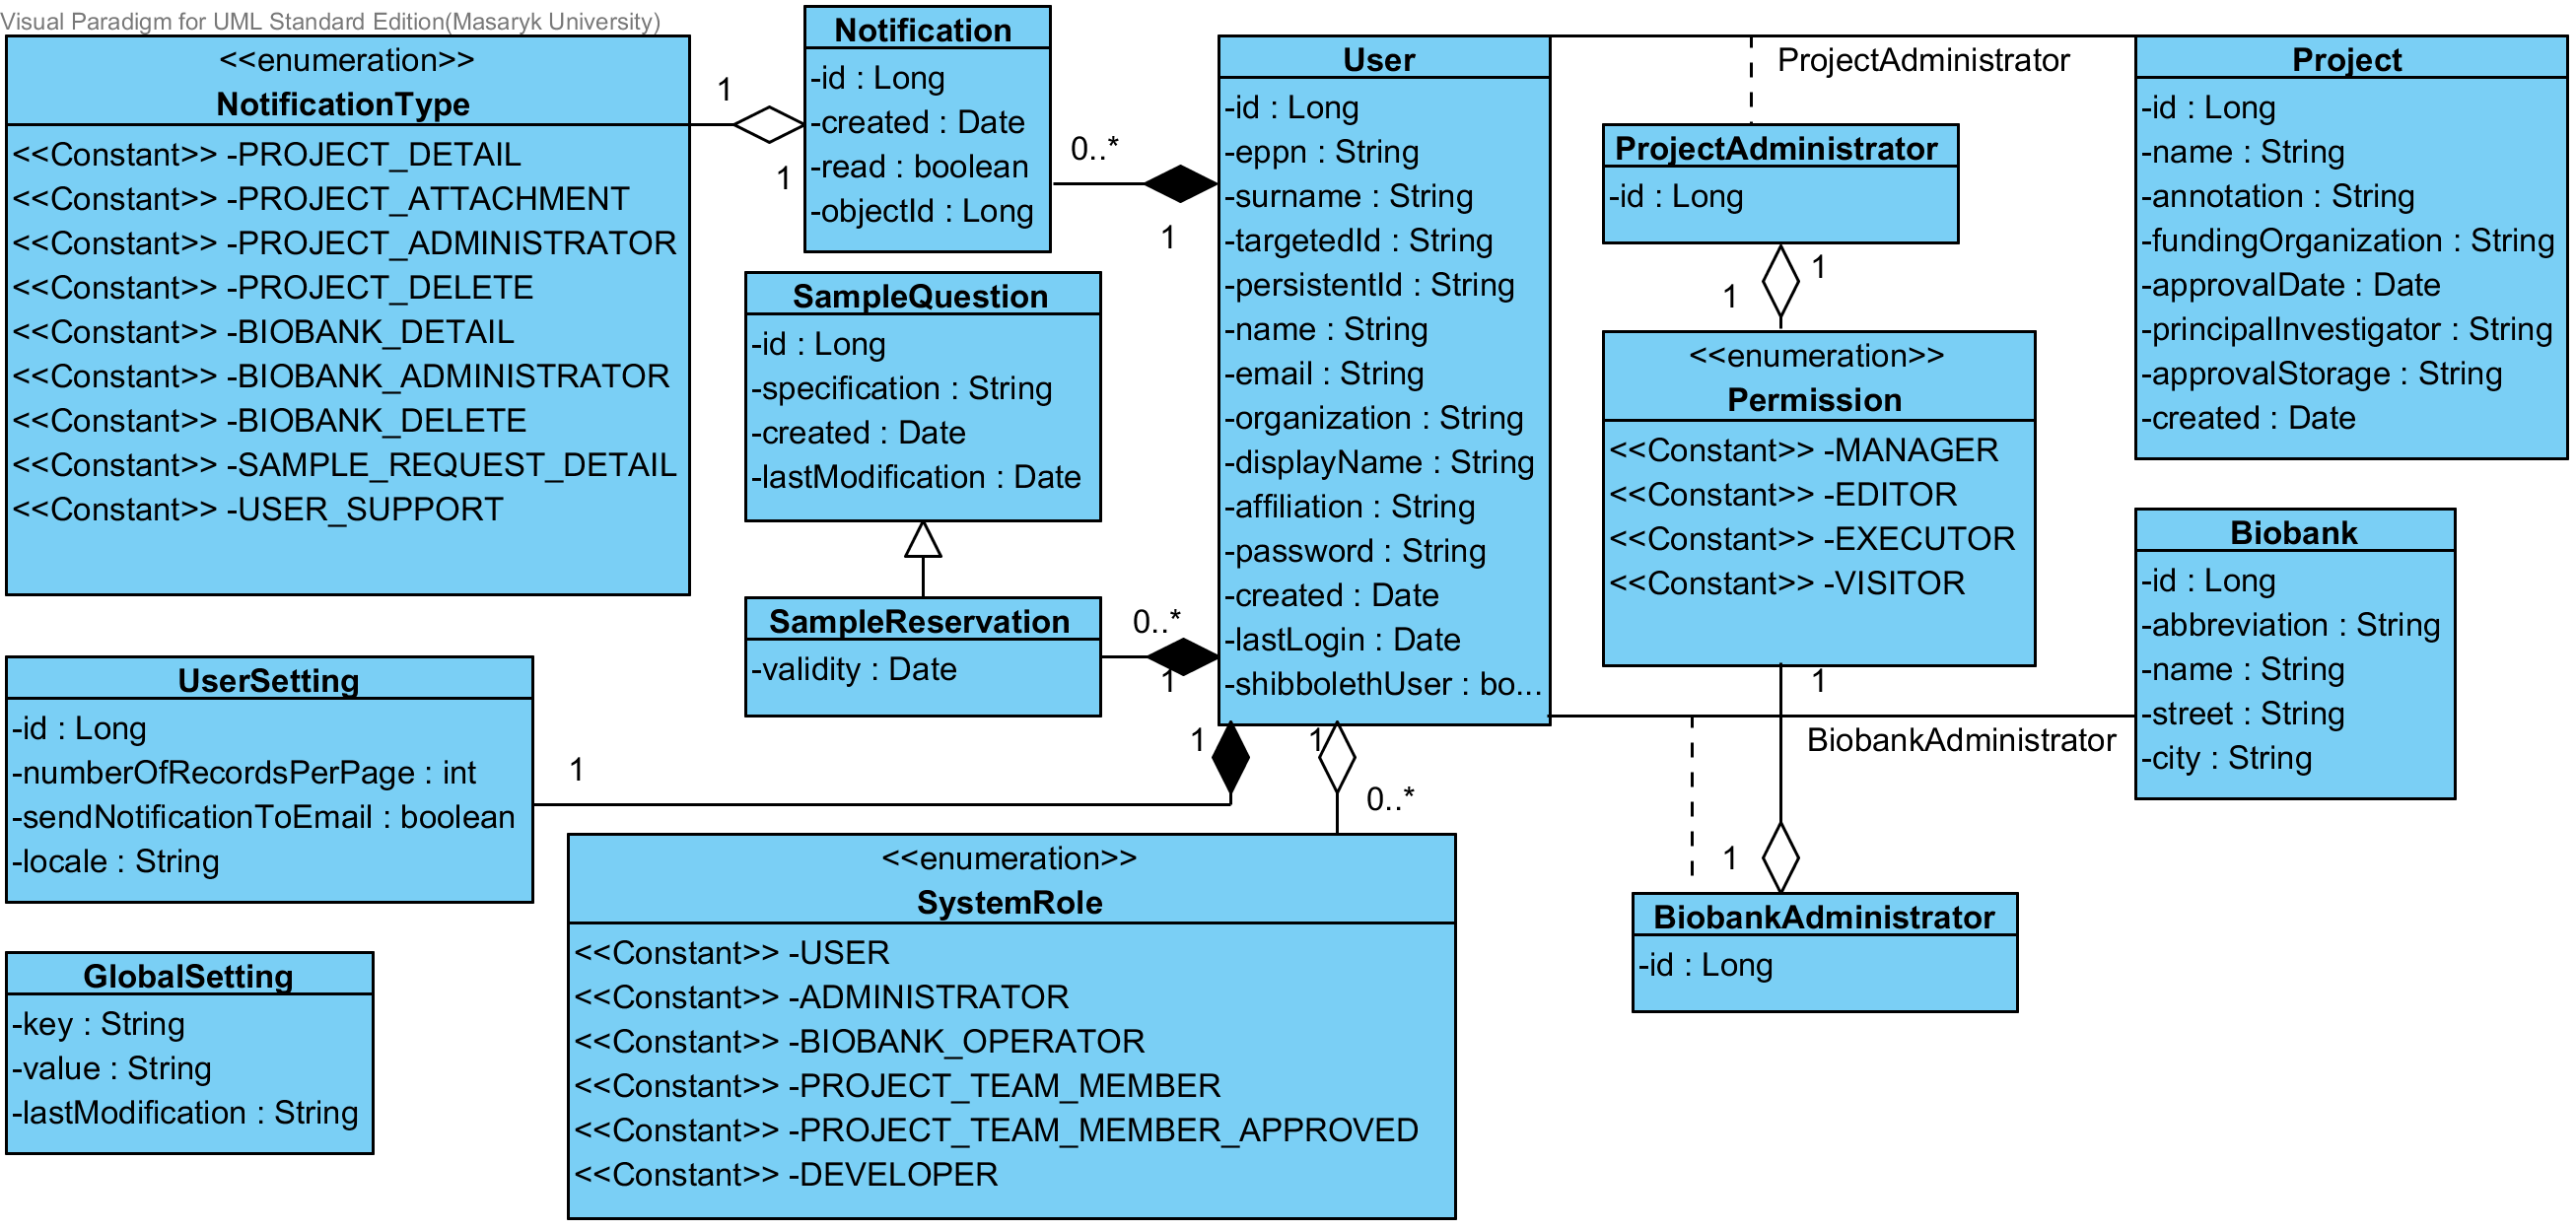
\includegraphics[width=\textwidth]{UserView}
\caption{UML class diagram tříd souvisejících s uživatelem}
\label{fig:index:uml:class:user}
\end{center}
\end{figure}


\section{Projekt}
Objekt \textit{Project} představuje záznam o existujícím podaném projektu. Většina ukládaných atributů vychází z formálních náležitostí související s existujícím projektovým záměrem:
\begin{compactitem}
	\item name -- název projektu,
	\item fundingOrganization -- kdo projekt financuje,	
	\item approvedBy -- kým byl projekt schválen. Schvalováním je v tomto kontextu myšlen proces mimo aplikaci - tj. nikoli formální kontrola administrátory \ProjectName
	\item approvalStorage -- kde je fyzický souhlas fyzicky uložen,
	\item principalInvestigator -- hlavní řešitel projektu. Položka je ukládána jako obyčejné textové pole pro případ, že by dotyčná osoba nebyla autorizovaná k přístupu do systému (např. zaměstnanec instituce nezačleněné do eduId).
	\item homeInstitution -- instituce, která projekt zaštiťuje,
	\item approvalDate -- datum schválení projektového záměru,
	\item annotation -- textový popis projektového záměru.
\end{compactitem}
Všechny jmenované atributy kromě anotace jsou považované za konstatní v průběhu životního cyklu projektu. Ostatní atributy souvisí s aplikační logikou. 

\begin{figure}[h!]
\begin{center}
	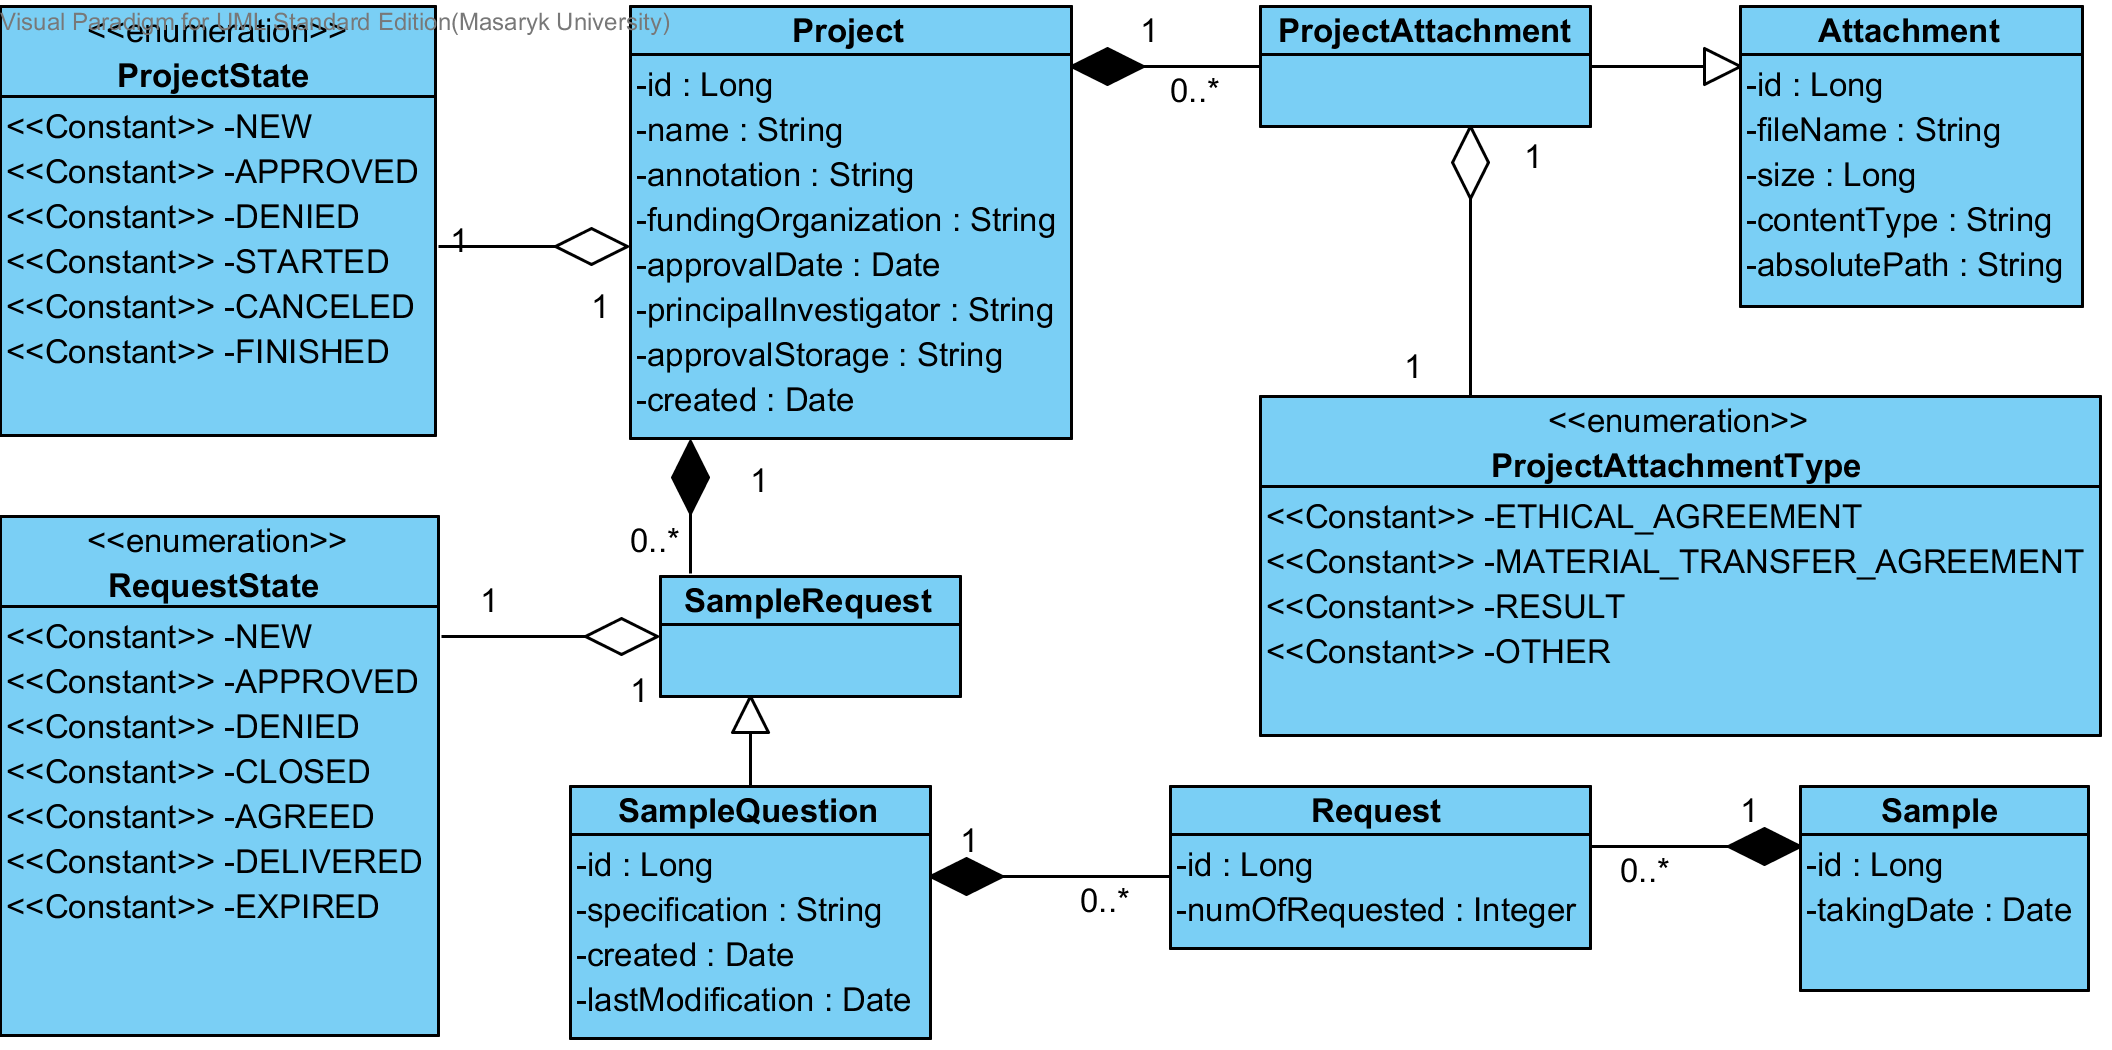
\includegraphics[width=\textwidth]{ProjectView}
\caption{UML class diagram tříd souvisejících s projektem}
\label{fig:index:uml:class:project}
\end{center}
\end{figure}

\subsection{Příloha}
Při nahrání projektu je nutné nahrát podepsaný formulář MTA. Model aplikace umožňuje, aby bylo nahráno libovolné množství příloh k projektu. Pro každou přílohu je možné definovat jaký je její význam v rámci projektu pro snazší organizaci. U kategorizace příloh se nepočítá s velkými změnami, takže byl pro jejich definování použit výčtový typ.

\subsection{Životní cyklus projektu}
Po založení je projekt označen jako \textit{nový}. Po kontrole formálních náležitostí administrátorem může být \textit{schválen} nebo \textit{zamítnut}. V kontextu schváleného projektu je již možné žádat o vzorky. Projekt s alespoň jednou žádostí je považován za \textit{zahájený}. Na konci realizace lze označit projekt za \textit{dokončený}. Ten v systému i nadále zůstává pro archivaci, ale je již pouze pro čtení a nelze v jeho kontextu žádat o vzorky. 
V aplikaci je definována i možnost zrušit schválený projekt (\textit{cancel}). Tato funkce, ale není ve stávající verzi zpřístupněna na uživatelském webovém rozhraní. Životní cyklus projektu je znázorněn na diagramu \ref{fig:implementace:projekt:cyklus}. Barevně jsou znázorněny události iniciované {\color{palatinatepurple}administrátory} a {\color{cyan}členem projektového týmu}. 

\begin{figure}[hbtp]
\begin{center}
\begin{tikzpicture}[->,>=stealth',shorten >=1pt,auto,node distance=45mm,
  thick,main node/.style={ellipse,draw}]

  \node[main node] (novy) {Nový};
  \node[main node] (schvaleny) [right of=novy] {Schválen};
  \node[main node] (zamitnuty) [below = 20mm of schvaleny] {Zamítnut};
  \node[main node] (zapocaty) [right of=schvaleny] {Započat};
  \node[main node,  dashed] (zruseny) [below = 20mm of zapocaty] {Zrušen};
  \node[main node] (dokonceny) [right of=zapocaty] {Dokončen};

  \path[every node/.style={font=\sffamily\small}]
    (novy) 
        edge [right, palatinatepurple] node[sloped, above] {Schválit} (schvaleny)
        edge [right, palatinatepurple] node[sloped, above] {Zamítnout} (zamitnuty)
    (schvaleny)
    	edge [right, cyan] node[sloped, above] {Žádost} (zapocaty)
        edge [bend left, cyan] node[sloped, above] {Dokončit} (dokonceny)
        edge [bend left, dashed, palatinatepurple] node[right] {Zrušit} (zruseny)
    (zamitnuty)
	(zapocaty)
     	edge [right, cyan] node[sloped, above] {Dokončit} (dokonceny)
        edge [bend left, dashed, palatinatepurple] node[right] {Zrušit} (zruseny)
    (zruseny)
    (dokonceny);

\end{tikzpicture}
\caption{Životní cyklus projektu}
\label{fig:implementace:projekt:cyklus}
\end{center}
\end{figure}

\subsection{Životní cyklus žádosti a rezervace o vzorků}
Uživatel s projektovým záměrem, ale bez splněných formálních náležitostí, může podat žádost o rezeraci vzorků. Ta je \textit{schválena} v situaci, kdy banka má kapacitu na to, aby žádosti vyhověla (tj. mají dostatek vzorků). Jinak je rezervace \textit{zamítnuta}. Ke schválené rezervaci je možné přiřadit konkrétní počty alikvoty vzorků. Když je seznam vzorků kompletní, je žádost \textit{uzavřena}. Od chvíle uzavření běží lhůta platnosti rezervace. Když tato lhůta vyprší, tak je žádost označena jako \textit{expirována} a alokované vzorky jsou uvolněny.
Źádost lze přiřadit k vybranému, schválenému projektu, ke kterému má uživatel oprávnění spravovat žádosti i vzorky. Tím je možné se vyhnout propadnutí rezervace. 
Na základě pouhé rezervace není možné fyzické vzorky získat. Životní cyklus rezervace je znázorněn v diagramu \ref{fig:implementace:rezervace:cyklus}, zatímco cyklus žádosti je v diagramu \ref{fig:implementace:zadost:cyklus}. Pro oba diagramy platí barevné odlišení iniciátorů znázorněných událostí: {\color{palatinatepurple}administrátor biobanky}, {\color{cyan}uživatel}/{\color{cyan}člen projektového týmu}. 

\begin{figure}[hbtp]
\begin{center}
\begin{tikzpicture}[->,>=stealth',shorten >=1pt,auto,node distance=45mm,
  thick,main node/.style={ellipse,draw}]

  \node[main node] (novy) {Nová};
  \node[main node] (schvalen) [right of=novy] {Schválena};
  \node[main node] (zamitnut) [below = 20mm of schvalen] {Zamítnuta};
  \node[main node] (uzavren) [right of=schvalen] {Uzavřena};
  \node[main node] (expirovan) [right of = uzavren] {Expirována};
	\node[main node] (zadost) [below = 20mm of uzavren] {Žádost};
    
  \path[every node/.style={font=\sffamily\small}]
    (novy)
    	edge [right, palatinatepurple] node[sloped, above] {Schválit} (schvalen)
      edge [right, palatinatepurple] node[sloped, above] {Zamítnout} (zamitnut)
    (schvalen)
    	edge [right, palatinatepurple] node[sloped, above] {Zkompletovat} (uzavren)
    (zamitnut)
    (uzavren)
      edge [right] node[sloped, above] {Expirace} (expirovan)
			edge [right] node[right, cyan] {Přiřadit projektu} (zadost);
\end{tikzpicture}
\caption{Životní cyklus rezervace}
\label{fig:implementace:rezervace:cyklus}
\end{center}
\end{figure}

Počátek životního cyklu žádosti o vzorky je totožný s rezervací. V situaci, kdy je žádost uzavřena pracovníkem biobanky je umožneno rozhodnutí žadateli, zda je sada vzorků dostačující. Tato volba je zde pro situaci, kdy vzorky nesplňují kladené požadavky. Žádost se tím vrátí do stavu \textit{schválena}, aby bylo opět možné editovat sadu vzorků.
Může také nastat situace, že o stejné vzorky bylo požádáno ve více biobankách a více žádostí bylo vyřízeno kladně, takže je pro projekt alokováno více zdrojů než je nutné. V této situaci se může správce projektu žádost smazat a tím alokované vzorky uvolnit.
Po schválení vybrané sady žadateli jsou tyto vzorky fyzicky připraveny k odebrání. Žádost, s fyzicky předanými vzorky je označena jako \textit{doručena}.

\begin{figure}[hbtp]
\begin{center}
\begin{tikzpicture}[->,>=stealth',shorten >=1pt,auto,node distance=45mm,
  thick,main node/.style={ellipse,draw}]

  \node[main node] (novy) {Nová};
  \node[main node] (schvalen) [right of=novy] {Schválena};
  \node[main node] (zamitnut) [below = 20mm of schvalen] {Zamítnuta};
  \node[main node] (uzavren) [right of = schvalen] {Uzavřena};
  \node[main node] (potvrzen) [right of = uzavren] {Potvrzena};
  \node[main node] (vydan) [below = 20mm of potvrzen] {Předáno};
    
  \path[every node/.style={font=\sffamily\small}]
    (novy)
    	edge [right, palatinatepurple] node[sloped, above] {Schválit} (schvalen)
        edge [right, palatinatepurple] node[sloped, above] {Zamítnout} (zamitnut)
    (schvalen)
    	edge [right, palatinatepurple] node[sloped, above] {Zkompletovat} (uzavren)
    (zamitnut)
    	
    (uzavren)
    	edge [right, cyan] node[sloped, above] {Vyhovuje} (potvrzen)
        edge [bend left, cyan] node[sloped, above] {Nevyhovuje} (schvalen)
    (potvrzen) 
    	edge [right, palatinatepurple] node[right] {Předat} (vydan)
    ;

\end{tikzpicture}
\caption{Životní cyklus žádosti}
\label{fig:implementace:zadost:cyklus}
\end{center}
\end{figure}


\section{Biobanka}
Objekt reprezentující jednoho z partnerů, zapojených do projektu, který poskytuje biologický materiál ostatním. Atribut \textit{abbreviation} slouží k propojení exportů s konkrétní instancí třídy \textit{Biobank}.

\begin{figure}[h!]
\begin{center}
	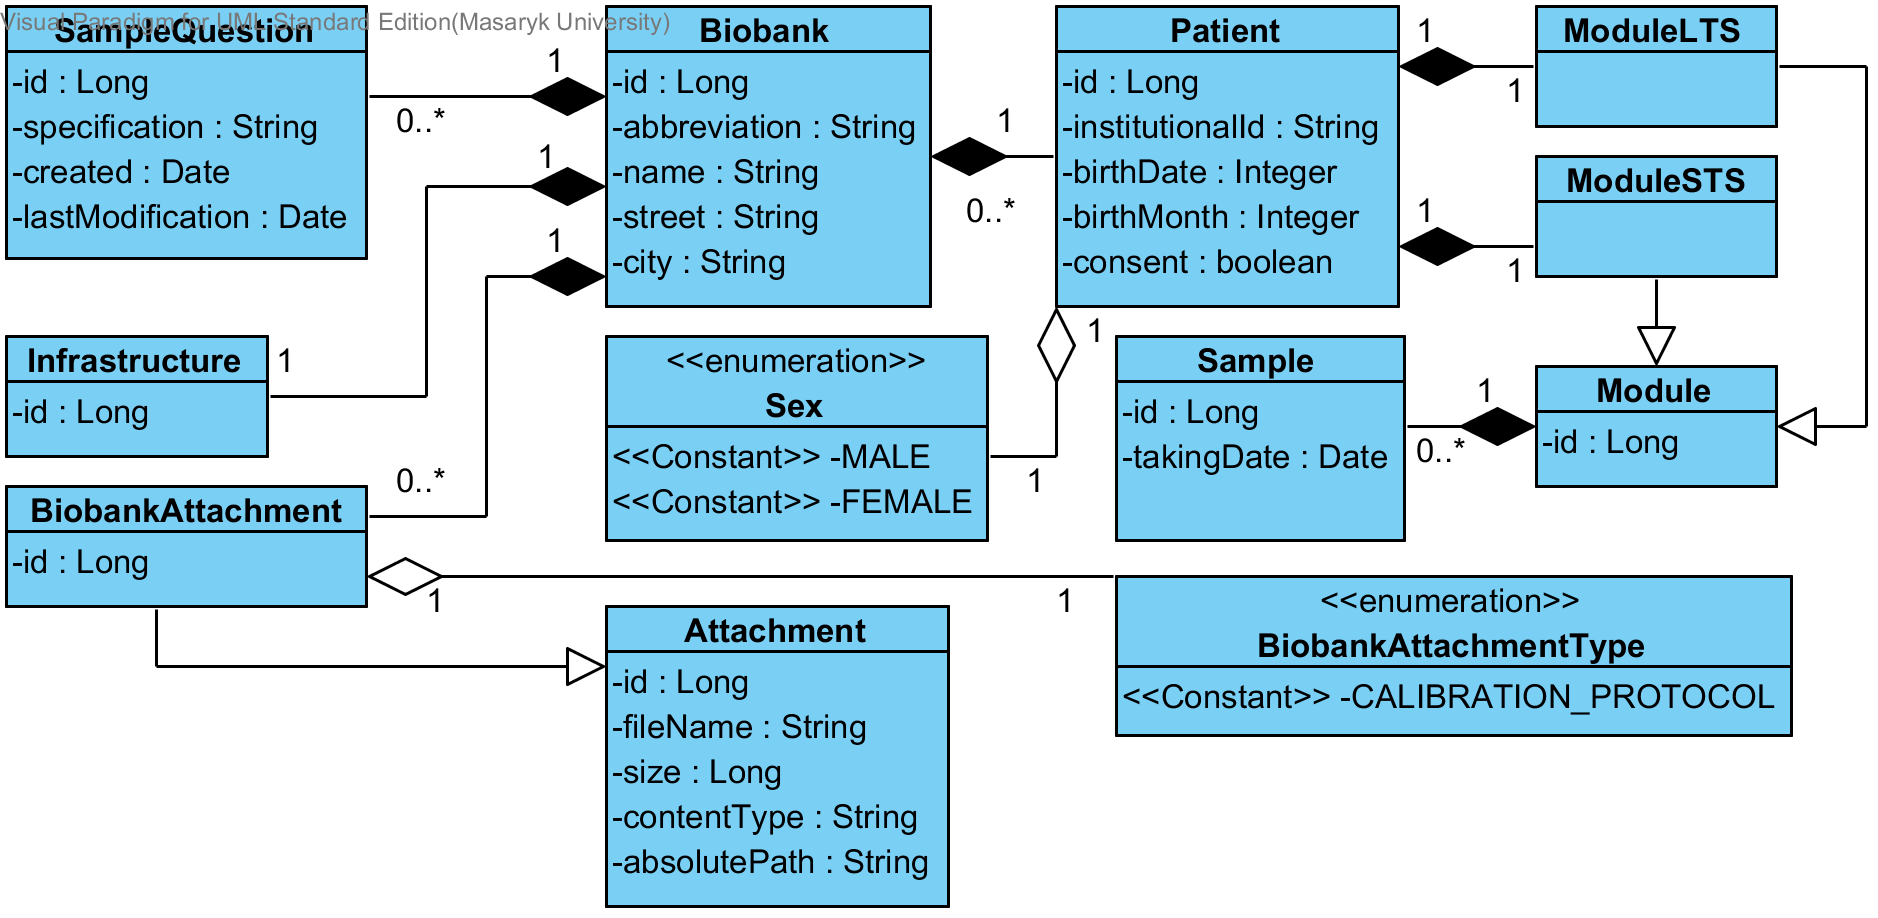
\includegraphics[width=\textwidth]{BiobankView}
\caption{UML class diagram tříd souvisejících s biobankou}
\label{fig:index:uml:class:biobank}
\end{center}
\end{figure}

\subsection{Infrastruktura biobanky}
Diagram \ref{fig:index:uml:class:infrastructure} popisuje, jakým způsobem je v aplikaci uložena struktura repozitáře biobanky. Struktura vychází z analýzy popsané v sekci \ref{chapter:analysis:subsection:monitoring}.

\begin{figure}[h!]
\begin{center}
	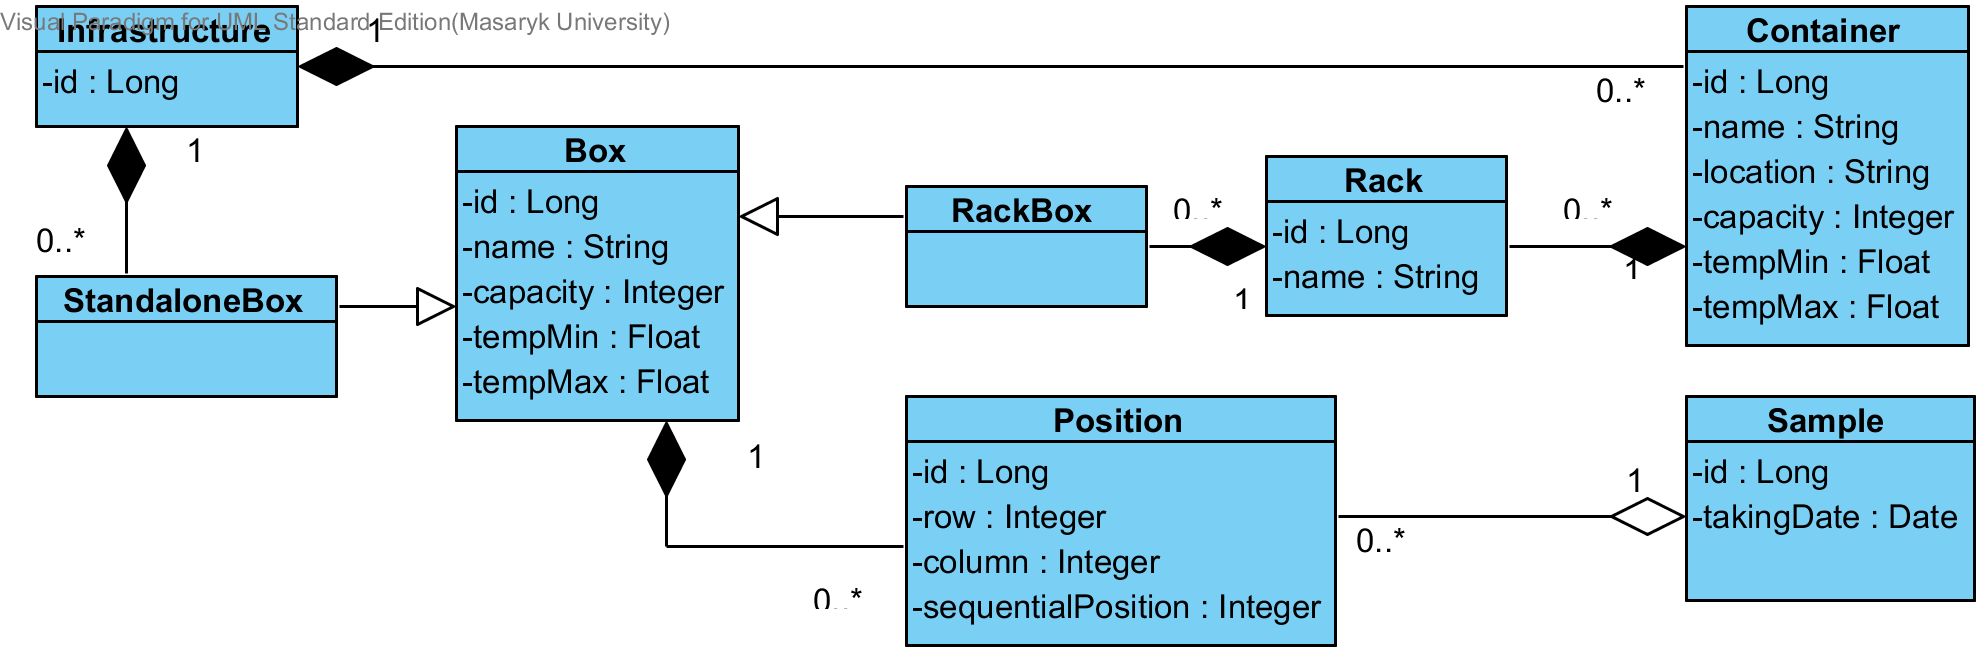
\includegraphics[width=\textwidth]{InfrastructureView}
\caption{UML class diagram popisující strukturu repozitáře}
\label{fig:index:uml:class:infrastructure}
\end{center}
\end{figure}

\subsection{Monitoring biobanky}

\section{Popis uložených vzorků}
Objektový návrh \ref{fig:index:uml:class:sample} vychází ze struktury exportu popsaném v části \ref{chapter:analysis:subsection:index} 

\begin{figure}[h!]
\begin{center}
	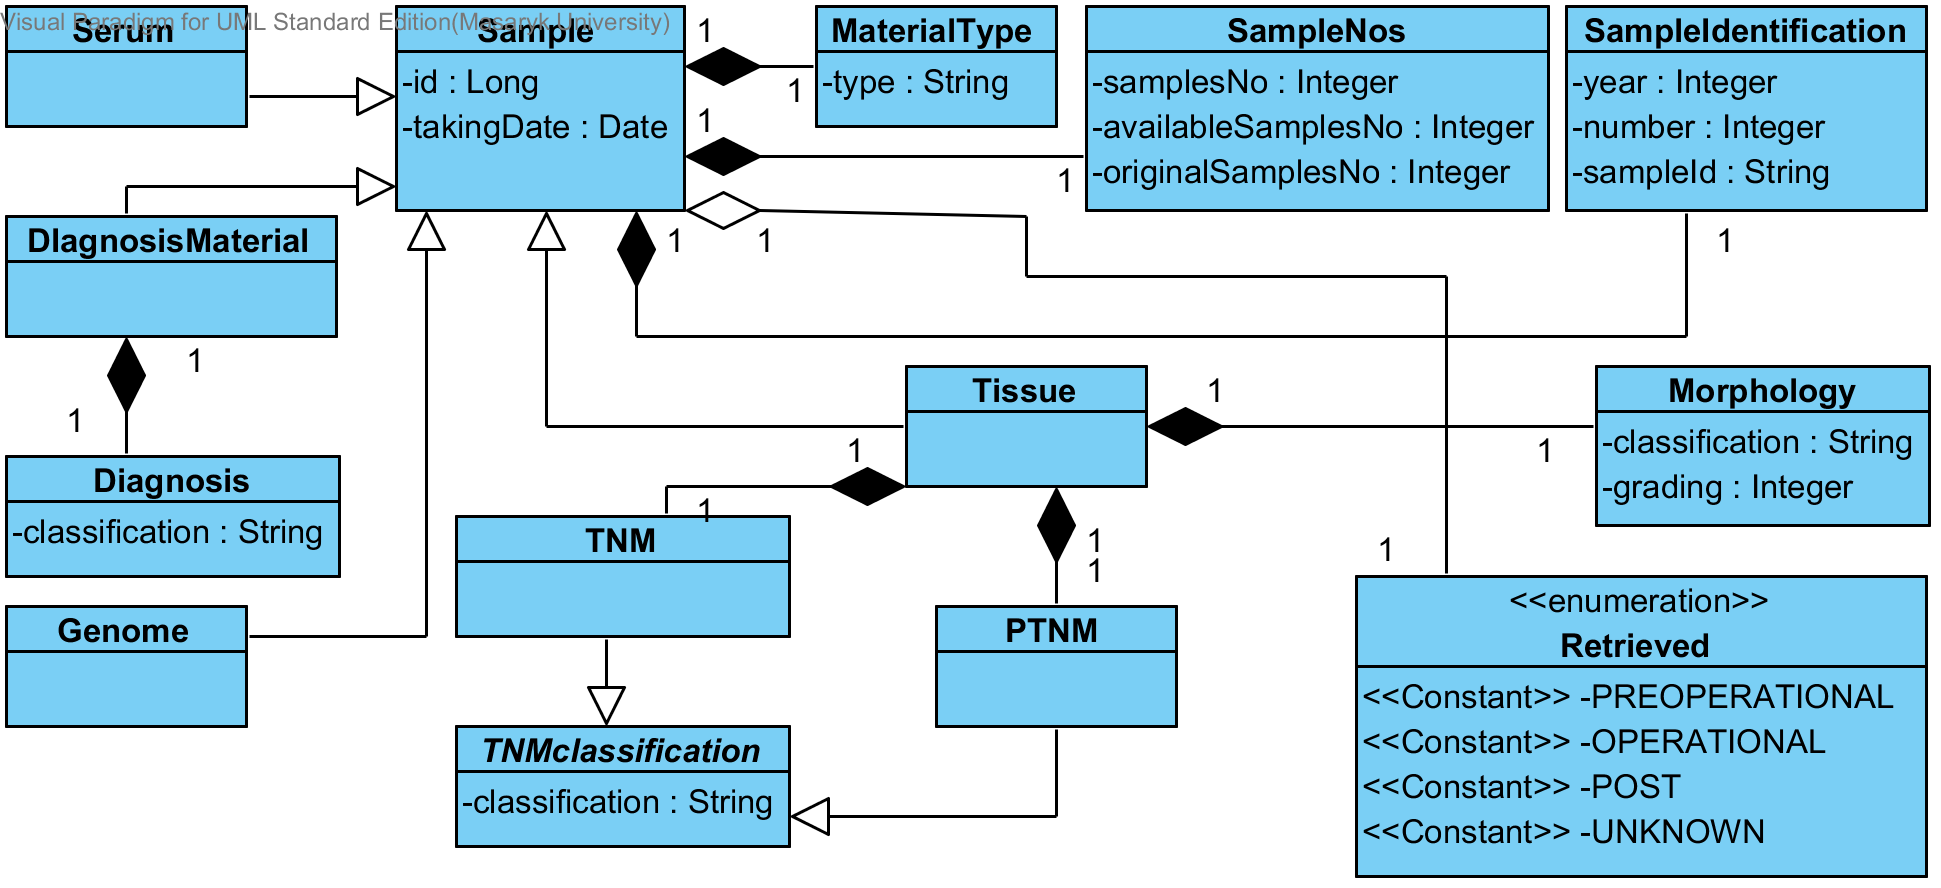
\includegraphics[width=\textwidth]{SampleView}
\caption{UML class diagram popisující biologický materiál}
\label{fig:index:uml:class:sample}
\end{center}
\end{figure}


\section{Autorizace uživatelů}
Pro stanovení které zdroje systému může uživatel používat byly stanoveny systémové role. Pro jemnější členění oprávnění vztažených ke konkrétnímu objektu byly definovány úrovně oprávnění.

\subsection{Systémové role}
Systémové role jsou definovány enumerační třídou cz.bbmri.entities.enumeration.SystemRole. 

\paragraph*{Uživatel} -- Implicitní role každého uživatele oprávněného přistupovat k indexu. Při autentizaci uživatele je na základě parametrů předávaných z eduId stanoveno zda může být dotyčnému uživateli umožněno vstoupit do systému - každý kdo je vpuštěn má roli \textit{uživatel}. Pohyb uživatele bez role \textit{uživatel} je považováno za chybu.
Uživateli s touto rolí je dovoleno:
\begin{compactitem}
	\item přistupovat ke svým vlastním údajům a k osobnímu nastavení
	\item podávat rezervace na vzorky
	\item nahrávat informace o projektech
	\item zobrazit kontakty na vývojáře a administrátory systému
	\item zobrazit všechny biobanky registrované v systému.
\end{compactitem}

\paragraph*{Správce biobanky} -- Každý uživatel s oprávněním alespoň k jedné biobance má systémovou roli \textit{správce biobanky}. Samotná systémová role upravuje pouze položky v menu. Autorizace pro provádění konkrétních operací je stanovena na základě oprávnění ke konkrétní instanci biobanky. 

\paragraph*{Člen projektového týmu} -- Každý uživatel s oprávněním alespoň k jednomu projektu má systémovou roli \textit{člen projektového týmu}. Obdobně jako u biobanky je i u projektu autorizace rozhodována pro každou instanci zvlášť podle oprávnění.

\paragraph*{Člen projektového týmu se schváleným projektem} -- Každý uživatel s oprávněním alespoň k jednomu schválenému projektu. Při schválení projektu nahrazuje roli \textit{člen projektového týmu}.
Uživateli s touto rolí je dovoleno:
\begin{compactitem}
	\item zobrazit monitoring teploty ve všech biobankách.
\end{compactitem}

\paragraph*{Vývojář} -- Uživatel pracující na vývoji systému. 
Uživateli s touto rolí je dovoleno:
\begin{compactitem}
	\item založit biobanku, smazat biobanku
	\item zobrazit veškeré informace zobrazované na webu bez možnosti editace
	\item přiřadit nebo odebrat uživateli roli vývojáře nebo administrátora.
\end{compactitem}

\paragraph*{Administrátor} -- Koordinátor projektu \ProjectName.
Uživateli s touto rolí je dovoleno:
\begin{compactitem}
	\item založit biobanku, smazat biobanku
	\item zobrazit veškeré informace zobrazované na webu bez možnosti editace
	\item přístup ke globálnímu nastavení systému
	\item přiřadit nebo odebrat uživateli roli vývojáře nebo administrátora.
\end{compactitem}


\subsection{Oprávnění k projektu}
V průběhu realizace se ukázalo, že je žádoucí, aby kardinalita mezi projektem a uživatelem nebyla n:1, ale n:m. Oprávnění k úpravě projektu, ale nemůže být vázané na systémovou roli, protože pak by při špatném rozvežení .jsp stránek hrozilo, že bude umožněna manipulace s cizím projektem. Z hlediska spolupráce více lidí na projektu je také vhodné umožnit delegování odpovědnosti. Tyto jmenované argumenty vedly k potřebě rozlišovat úroveň oprávnění přístupu zvlášt ke každému projektu.
Mezi jednotlivými oprávnění je vztah inkluze, tj. vyšší zahrnuje vše z nižšího. Oprávnění jsou definována v třídě cz.bbmri.entities.enumeration.Permission.
\paragraph*{Návštěvník (Visitor)} -- Uživateli s tímto oprávněním je umožněno zobrazit všechny stránky související s projektem, ke kterému se oprávnění pojí - tj. detail projektu, projektový tým, přílohy a další. Není mu ale umožněno data jakkoli měnit. Uživatel nenese žádnou odpovědnost za aktivitu v systému.
\paragraph*{Výkonný pracovník (Executor)} -- Oprávnění \textit{executor} umožňuje uživateli vykonávat následující operace s projektem:
\begin{compactitem}
	\item označit projekt jako dokončený
	\item pracovat s žádostmi o vzorky (vytvoření, schvalování, ...)
	\item manipulace s přílohami projektu
\end{compactitem}

\paragraph*{Pracovník s možností editace (Editor)} -- Uživatel s oprávněním \textit{editor} může měnit editovatelná pole související s projektem.
\paragraph*{Manager} -- Nejvyšší opravnění umožňující manipulovat se složením týmu a s oprávněním jednotlivých osob.


\subsection{Oprávnění k biobance}
Stejná motivace jako u projektu vedla k zavedení úrovní oprávnění i pro biobanky. Oprávnění jsou definována následovně. 
\paragraph*{Návštěvník (Visitor)} -- Implicitní oprávnění. Uživateli s tímto oprávněním je umožněno zobrazit všechny stránky související s biobankou.
\paragraph*{Výkonný pracovník (Executor)} -- Uživatel s oprávněním \textit{executor} může:
\begin{compactitem}
	\item schvalovat projekty
	\item manipulace s žádostmi o vzorky
\end{compactitem}
\paragraph*{Pracovník s možností editace (Editor)} 
\begin{compactitem}
	\item manuální vytváření infrastruktury biobanky (kontejnery, stojany, ...)
	\item manuální vytváření pacientů a vzorků
	\item možnost měnit editovatelné položky biobanky
\end{compactitem}
\paragraph*{Manager} -- Nejvyšší opravnění umožňující manipulovat se složením týmu a s oprávněním jednotlivých osob.

% ------------------------------------------------------------------------      
% Implementace
\chapter{Implementace}
Aplikace je provozována na serveru Metacentra\footnote{http://www.metacentrum.cz/}, na adrese http://cloud19.cerit-sc.cz. Pro testovací účely byl vyhrazen druhý server http://cloud20.cerit-sc.cz. V obou případech se jedná o linuxové stroje s operačním systémem \textit{Debian Squeeze} verze 6.0. Stroje jsou vybaveny procesory Intel Xeon E312xx Sandy Bridge a disponují 6GB operační paměti.
Pro ostré nasazení aplikace byly zaregistrovány domény www.bbmri.cz a index.bbmri.cz, které odkazují na produkční server cloud19.cerit-sc.cz. Domény jsou ve správě informatického oddělení MOÚ.
Dle požadavků bylo nutné, aby bylo nutné zajistit šifrování komunikace se serverem. Proto byl pro uvedené domény vystaven certifikát, používaný pro https. 
Doména bbmri.cz má čistě informační charakter, zatímco doména https://index.bbmri.cz vede do vlastní aplikace.
Pro vývoj aplikace byl používán repozitář github\footnote{Adresa repozitáře: \url{https://github.com/Ondrej-vojtisek/bbmri}}. 
Cílem této kapitoly je seznámit čtenáře s některými použitými technologiemi a vysvětlit některé nestandardní implementační detaily.

% ------------------------   
% Section 
\section{Použité technologie}
Cílem této kapitoly je stručně představit použité technologie a prezentovat argumenty pro jejich výběr, pokud existují. 
Aplikace je implementována v Javě verze 7, nicméně nevyužívá žádných syntaktických \uv{novinek} Javy 7 a kód beze změn funguje i pro Javu 6. 

\subsection{Maven}
Pro sestavení aplikace byl používán nástroj Maven\footnote{http://maven.apache.org/}. Programátor v souboru pom.xml nadefinuje, které knihovny a programovací nástroje aplikace používá, včetně specifikace verze těchto nástrojů. Maven tyto závislosti stáhne a aplikaci sestaví. Pro vývoj představuje použití mavenu usnadnění, protože vývojář nemusí řešit tranzitivní závislosti jednotlivých knihoven a má lepší přehled nad verzemi použitých knihoven. 

\subsection{Hibernate}
Pro ukládání dat a pro přístup k nim byl použit ORM (Object-Relational Mapping\footnote{Způsob konverze dat mezi relační databází a objektem objektově orientovaného jazyka.}) JPA (Java Persistence API). JPA je rozhraní (API), které definuje jakým způsobem jsou objekty mapovány na tabulky relační databáze. Vazby mezi entitami aplikace jsou definovány pomocí anotací. Parametry připojení k databázi jsou JPA poskytnuty konfiguračními soubory\footnote{Parametry připojení definuje soubor \textit{persistence.xml}.}. JPA není závislé na nezávislé na implementaci databáze.
Hibernate je implementace JPA, která byla v aplikaci použita. Konkrétně byla použita verze 3.6.10. Alternativou k Hibernate je např. OpenJPA\footnote{https://openjpa.apache.org/}. Argumentem pro volbu Hibernate byl explicitní požadavek v zadání práce, stanovený s cílem sjednotit používané technologie v projektech realizovaných na ÚVT MUNI (resp. v centru CERIT-SC). 
Hibernate za vývojáře zajišťuje vytvoření schéma databáze podle datového modelu (popsaného anotacemi entit aplikace). Databáze je vytvářena automaticky a bez nutnosti zásahu programátora jsou do databáze propagovány všechny případné změny entit. 
Pro dotazování na databázi se používá JPQL (Java Persistence Query Language) namísto běžného SQL používaného v relačních databázích. JPQL umožňuje pokládat dotazy na základě znalosti entit a do bez znalosti jejich skutečného uložení v databázi (např. kladení dotazů bez znalosti pojmenování tabulek).

\subsection{Spring}
Jako základ pro implementaci aplikační vrstvy aplikace byl použit aplikační rámec Spring\footnote{http://spring.io/}, který umožňuje automatické dynamické vytváření potřebných objektů za běhu aplikace. Tento mechanismus se nazývá \textit{dependency injection} a pro programátora představuje usnadnění, neboť se nemusí zabývat inicializací objektů. Objekty, jejichž závislost má spravovat Spring jsou v kódu označeny anotací \textit{@Autowired}.
Alternativou pro Spring je aplikační rámec EJB (Enterprise Java Beans).

\subsection{Stripes}


Stripes, JPA, Hibernate, bootstrap, postgres, apache, tomcat, shibboleth, 
git, jquery, použité jquery knihovny, xpath, Spring, ... 

\section{Použité javascriptové a Jquery knihovny}
\subsection{bootstrap}

\section{Logování}

\section{Nastavení serveru}

\subsection{Uživatelé}
\ovnote{definovaní uživatelé a skupiny systému?}

\subsection{Firewall}
Pro zajištění základní bezpečnosti serveru byl nastaven firewall s následujícími pravidly:
\ovnote{nastavit, vypsat, případně nechat v appendixu}

\subsection{Shibboleth}
Pro autentizace uživatelů byla aplikace zapojena do federace eduId, která je implementována pomocí Shibbolethu. Pro nastavení bylo nutné nainstalovat příslušné balíčky a nastavit konfiguraci této služby.
\ovnote{konfigurace v apendixu?}

\subsection{Aktualizace času}
Pro korektní běh shibbolethu je nutná časová synchronizace mezi serverem a poskytovatelem identiti (IdP). Z toho důvodu je nezbytně nutné nastavit pravidelnou aktualizaci hodin. 
\subsection{Apache, Tomcat}
\ovnote{konfigurace v apendixu?}

\section{Práva k~využívání převzatých částí kódu}
\ovnote{Zmínit, které části kódu jsou převzaté a jaké jsou k nim práva}

\section{Testování}
Aplikace byla testována na několika úrovních, různými způsoby. Pro entity obsahující složitější metody, které bylo nezbytné testovat, byly implementovány jednoduché jednotkové testy. 

Druhou testovanou úrovní byly testy DAO tříd. Ty slouží k otestování správnosti anotací entit (anotace pro Hibernate definující kardinalitu vztahů), dále k otestování metod a dotazů kladených na databázi. Pro implementaci těchto testů je použit nový konfigurační soubor pro Spring, který pracuje s databází drženou v paměti, tak aby nebylo nutné vracet skutečnou databázi po testech do původního stavu. Jako databáze byla použita HSQLDB (HyperSQL DataBase).

Další fází testování bylo ověřit funkci aplikační (servisní) vrstvy. Aby bylo možné testovat pouze funcionalitu aplikační vrstvy bez vlivu na nižší závislosti, jsou v testech použity tzv. mock objekty. Ty slouží k simulaci chování DAO vrstvy, takže testy ověřující výhradně chování aplikační vrstvy.

Pro manuální testování webového rozhraní je použita možnost lokálních uživatelských účtů, tak aby bylo možné se k aplikaci přihlásit, bez konfigurace lokálního IdP pro Shibboleth. Tento způsob přihlášení do aplikace není při ostrém chodu aplikace vůbec povolen.

\section{Další vývoj}
Aplikaci čeká v budoucnu ještě mnoho proměn. Dá se očekávat, že při prvních měsících reálného využívání se teprve objeví mnoho nových požadavků na rozšíření datového modelu. Zcela zásadní změnou změnou by pak aplikaci musela projít při zapojení \ProjectName do celoevropské BBMRI infrastruktury. Kromě těchto těžko předvídatelných změn by aplikace mohla být do budoucna rozšířena nebo zlepšena v následujících oblastech:

\paragraph*{AJAX} -- umožnění dílčích změn bez nutnosti znovunačíst celou webovou stránku. Tato změna by posunula webové rozhraní blíže k dnešním standardům.
\paragraph*{Zasílání informací e-mailem} -- umožnit prostřednictvím nastavení, že se budou upozornění zasílat emailem. Obdobně rozesílat e-mailem informace pro vývojáře o detekovaných chybách v systému.
\paragraph*{Podpora SVG} -- využít SVG k názornějšímu zobrazení jednotlivých prvků infrastruktury biobank.


% ------------------------------------------------------------------------      
% Závěr
\chapter{Návod}

\section{Konfigurace systému}
\ovnote{uživatel vs. vývojář vs. administrátor}

% ------------------------------------------------------------------------      
% Závěr
\chapter{Závěr}
Zmínit to, že jsem se technologie průběžně učil což mělo veliký efekt na časté zásadní změny v kódu práce. Přidat referenci na statistiky githubu.

%% Lists of tables and figures, glossary, etc.
%\printindex
%\printglossary
%\listoffigures
%\listoftables

%% Bibliography from references.bib
%\begingroup
%\def\tmpchapter{0}
%\renewcommand{\chaptername}{}
%\renewcommand{\thechapter}{}
%\addtocontents{toc}{\setcounter{tocdepth}{-1}}
%\chapter{Zdroje}
%\renewcommand{\chapter}[2]{}% for other classes

% Následují další kapitoly a podkapitoly, popřípadě závěr, dodatky, 
% seznam literatury či použitých obrázků nebo tabulek.

% LaTeX magic :) Při kopírování některé znaky chybí !!!!!
\renewcommand{\UrlBreaks}{\do\/\do\a\do\b\do\c\do\e\do\f\do\i\do\j\do\k\do\l\do\m\do\n\do\o\do\q\do\r\do\s\do\u\do\v\do\w\do\x\do\y\do\z\do\A\do\B\do\C\do\D\do\E\do\F\do\G\do\H\do\I\do\J\do\K\do\L\do\M\do\N\do\O\do\P\do\Q\do\R\do\S\do\T\do\U\do\V\do\W\do\X\do\Y\do\Z\do\?\do\=\do\-\do\0\do\1\do\3\do\4\do\5\do\6\do\7\do\8\do\9\do\p\do\d\do\h}
\mathchardef\UrlBreakPenalty=50\relax
\bibliographystyle{plainnat} %./splncs}
\bibliography{references}

%\addtocontents{toc}{\setcounter{tocdepth}{2}}
%\endgroup

% Prostředí pro přílohy
\begin{appendix}

\chapter{Obsah přiloženého DVD}
\textbf{Dokumenty}
\begin{itemize}
	\item Dokument popisující architekturu systému viz. \cite{ARCH_2014_1_25}
\end{itemize}

\chapter{Návod k instalaci na serveru}

\chapter{Číselníky jednotlivých institucí}

\section{LF~UP}

Biobanka LF~UP používá interně strukturování do archivačních řad v~následující struktuře:\\ \textbf{Pacient, odběr} 

	\begin{compactitem}
	\item Buňky 
		\begin{compactitem}
			\item BD, BE, LB, BO, BS, BU, BZ, LT, TR, KB, KK, PR
		\end{compactitem}

	\item Dusík 
		\begin{compactitem}
			\item TD
		\end{compactitem}

	\item DNA 
		\begin{compactitem}
			\item DG, DK, DM, DW
		\end{compactitem}

	\item Amplikon 
		\begin{compactitem}
			\item DA, DP
		\end{compactitem}

	\item Plazma/sérum 
		\begin{compactitem}
			\item KE, KP
		\end{compactitem}

	\item RNA 
		\begin{compactitem}
			\item RC, RV
		\end{compactitem}

	\item Řezy 
		\begin{compactitem}
			\item PP
		\end{compactitem}

	\item Sklíčka RT 
		\begin{compactitem}
			\item PS
		\end{compactitem}

	\item Sklíčka zamražená 
		\begin{compactitem}
			\item RY, NC, NR, BC
		\end{compactitem}
	\end{compactitem}

\begin{table}[ht] 
\centering
\begin{tabular}{l l}
\hline 
Typ materiálu & Kód \\
\hline \hline
buněčná suspenze 									& BS \\
DNA genomická 										& DG \\
DNA komplementární 								& DK \\
DNA whole genome amplified 				& DW \\
kostní dřeň nativní a nesrážlivá 	& RN \\
krev nesrážlivá 									& KN \\
krev plazma 											& KP \\
krev sérum 												& KE \\
krev srážlivá 										& KA \\
laváž 														& LA \\
likvor 														& LI \\
moč 															& MO \\
nátěr buněčný 										& NB \\
nátěr chromozomální 							& NC \\
nátěr kostní dřeň 								& NK \\
šťáva pankreatická  							& SP \\
parafinový blok 									& PB \\
parafinový řez 										& PR \\
RNA 															& RN \\
tkáň nativní 											& TN \\
tkáň RNA later 										& TR \\
tkáň zamražená 										& TZ \\
výpotek 													& VY \\

\hline %inserts single line 
\end{tabular} 
\caption{Číselník materiálů využívaný biobankou 1.~LF~UP}
\label{tab:ciselnik-mat-UP} % is used to refer this table in the text 
\end{table} 

\section{1.LF}

\begin{table}[ht] 
\centering
\begin{tabular}{l l}
\hline 
Typ materiálu & Kód \\
\hline \hline
Nádor maligní 							& Tm 	\\
Metastáza 									& Te 	\\
Nádor benigní 							& Tb 	\\
Zdravá tkáň 								& Th 	\\
Patol. tk. 									& Tp 	\\
Nádor nejisté biol. povahy 	& Tn 	\\
Carcinoma in situ 					& Ti 	\\
Suffix pro later 						& -L 	\\
Sérum 											& S~	\\
Plazma 											& P 	\\
Genomová DNA 								& G 	\\
Plná krev 									& B 	\\
Moč 												& U~	\\

\hline %inserts single line 
\end{tabular} 
\caption{Číselník materiálů využívaný biobankou 1.~LF~UK.}
\label{tab:ciselnik-mat-Ilfuk} % is used to refer this table in the text 
\end{table} 

\end{appendix}


%% End of the whole document
\end{document}